%%% Hlavní soubor. Zde se definují základní parametry a odkazuje se na ostatní části. %%%

%% Verze pro jednostranný tisk:
% Okraje: levý 40mm, pravý 25mm, horní a dolní 25mm
% (ale pozor, LaTeX si sám přidává 1in)
\documentclass[12pt,a4paper]{report}
\setlength\textwidth{145mm}
\setlength\textheight{247mm}
\setlength\oddsidemargin{15mm}
\setlength\evensidemargin{15mm}
\setlength\topmargin{0mm}
\setlength\headsep{0mm}
\setlength\headheight{0mm}
% \openright zařídí, aby následující text začínal na pravé straně knihy
\let\openright=\clearpage

%% Pokud tiskneme oboustranně:
% \documentclass[12pt,a4paper,twoside,openright]{report}
% \setlength\textwidth{145mm}
% \setlength\textheight{247mm}
% \setlength\oddsidemargin{15mm}
% \setlength\evensidemargin{0mm}
% \setlength\topmargin{0mm}
% \setlength\headsep{0mm}
% \setlength\headheight{0mm}
% \let\openright=\cleardoublepage

%% Použité kódování znaků: obvykle latin2, cp1250 nebo utf8:
\usepackage[utf8]{inputenc}

%%%
%%%
%%% Ostatní balíčky
%%%
%%%
\usepackage{graphicx}
\usepackage{amsmath,amssymb,amsthm}
\usepackage{cite} % bibtex
\usepackage[usenames,dvipsnames]{xcolor} % color names
\usepackage{color} % \color
\usepackage{enumitem} % compact lists
%\usepackage{MnSymbol} % \cupdot


%% Balíček hyperref, kterým jdou vyrábět klikací odkazy v PDF,
%% ale hlavně ho používáme k uložení metadat do PDF (včetně obsahu).
%% POZOR, nezapomeňte vyplnit jméno práce a autora.
\usepackage[unicode]{hyperref}   % Musí být za všemi ostatními balíčky
\hypersetup{pdftitle=Dissections of triangles and distances of groups}
\hypersetup{pdfauthor=Michal Szabados}

%%% Vlastne makra

%%%
%%% Theorem environments
%%%
\theoremstyle{plain}% default
	\newtheorem{thm}{Theorem}[chapter]
	\newtheorem{lem}[thm]{Lemma}
	\newtheorem{prop}[thm]{Proposition}
	\newtheorem{cor}[thm]{Corollary}
	%\newtheorem*{KL}{Klein's Lemma}

\theoremstyle{definition}
	\newtheorem{defn}[thm]{Definition}
	\newtheorem{conj}[thm]{Conjecture}
	\newtheorem{exmp}[thm]{Example}
	\newtheorem{alg}[thm]{Algorithm}
	\newtheorem{prob-intro}{Problem}
	\newtheorem{conj-intro}{Conjecture}

\theoremstyle{remark}
	\newtheorem*{rem}{Remark}
	\newtheorem*{note}{Note}

%%%
%%% Custom commands
%%%
\newcommand{\Z}{\mathbb Z}
%\newcommand{\N}{\mathbb N}
\newcommand{\Q}{\mathbb Q}
\newcommand{\gdist}{\mathop{\mathrm{gdist}}}
\newcommand{\dist}{\mathop{\mathrm{dist}}}
\newcommand{\spb}{\mathop{\mathrm{spb}}}
\newcommand{\lcm}{\mathop{\mathrm{lcm}}}

%%%
%%% Todos and notes
%%%
\newcommand\todo[1]{{\color{red}#1}}
\newcommand\side[1]{\normalmarginpar\mbox{}\marginpar{\footnotesize\raggedright\hspace{0pt}\color{Green}\emph{#1}}}

%%%
%%% Custom framebox
%%%
\newdimen\vmez
\vmez2pt
\newdimen\hmez
\hmez2pt
\def\myframebox#1{%
\setbox0%
\hbox{\vrule
	\vbox{\hrule
		\vskip\vmez
		\hbox{\hskip\hmez #1\hskip\hmez}
		\vskip\vmez
	\hrule
	}%
\vrule
}%
{\everycr{}\tabskip0pt \ooalign{\phantom#1\cr \hss\hbox to0pt{\hss \vbox to0pt{\vss\box0 \vskip-\vmez\vskip-0.4pt}\hss}\hss}}%
}

%%%
%%% Compact equations
%%%
\newenvironment{cosyeqnarray}%
{\setlength{\belowdisplayskip}{4pt} \setlength{\belowdisplayshortskip}{4pt}
\setlength{\abovedisplayskip}{4pt} \setlength{\abovedisplayshortskip}{4pt}
\begin{eqnarray}}%
{\end{eqnarray}}%

\newcommand\cosyalign[1]
{{\setlength{\belowdisplayskip}{4pt} \setlength{\belowdisplayshortskip}{4pt}
\setlength{\abovedisplayskip}{4pt} \setlength{\abovedisplayshortskip}{4pt}
\begin{align}#1
\end{align}}}

\newcommand\cosyalig[1]
{{\setlength{\belowdisplayskip}{4pt} \setlength{\belowdisplayshortskip}{4pt}
\setlength{\abovedisplayskip}{4pt} \setlength{\abovedisplayshortskip}{4pt}
\begin{align*}#1
\end{align*}}}

%%%
%%% Tables
%%%
\renewcommand{\arraystretch}{1.2}
\setlength{\tabcolsep}{6pt}

\newcommand\M[1]{{\myframebox#1}}

%%%
%%% Shorter overline
%%%
\newcommand{\overbar}[1]{\mkern 1.5mu\overline{\mkern-1.5mu#1\mkern-1.5mu}\mkern 1.5mu}

%%%
%%% Compact lists
%%%
\newenvironment{cosyitemize}%
{\begin{itemize}[topsep=2pt,itemsep=2pt,parsep=2pt,partopsep=2pt]}%
{\end{itemize}}%

\newenvironment{cosyenumerate}%
{\begin{enumerate}[topsep=2pt,itemsep=2pt,parsep=2pt,partopsep=2pt]}%
{\end{enumerate}}%


%%% Drobné úpravy stylu

% Tato makra přesvědčují mírně ošklivým trikem LaTeX, aby hlavičky kapitol
% sázel příčetněji a nevynechával nad nimi spoustu místa. Směle ignorujte.
\makeatletter
\def\@makechapterhead#1{
  {\parindent \z@ \raggedright \normalfont
   \Huge\bfseries \thechapter. #1
   \par\nobreak
   \vskip 20\p@
}}
\def\@makeschapterhead#1{
  {\parindent \z@ \raggedright \normalfont
   \Huge\bfseries #1
   \par\nobreak
   \vskip 20\p@
}}
\makeatother

% Toto makro definuje kapitolu, která není očíslovaná, ale je uvedena v obsahu.
\def\chapwithtoc#1{
\chapter*{#1}
\addcontentsline{toc}{chapter}{#1}
}

\begin{document}

%%%
%%% Compact equations
%%%
%\setlength{\belowdisplayskip}{4pt} \setlength{\belowdisplayshortskip}{4pt}
%\setlength{\abovedisplayskip}{4pt} \setlength{\abovedisplayshortskip}{4pt}


% Trochu volnější nastavení dělení slov, než je default.
\lefthyphenmin=2
\righthyphenmin=2

%%% Titulní strana práce

\pagestyle{empty}
\begin{center}

\large

Charles University in Prague

\medskip

Faculty of Mathematics and Physics

\vfill

{\bf\Large MASTER THESIS}

\vfill

\centerline{\mbox{
\includegraphics[width=60mm]{./img/logo.pdf}}}

\vfill
\vspace{5mm}

{\LARGE Michal Szabados}

\vspace{15mm}

% Název práce přesně podle zadání
{\LARGE\bfseries Dissections of triangles and distances of groups}

\vfill

% Název katedry nebo ústavu, kde byla práce oficiálně zadána
% (dle Organizační struktury MFF UK)
Department of Algebra

\vfill

\begin{tabular}{rl}

Supervisor\,of\,the\,master\,thesis: & prof.\,RNDr.\,Aleš Drápal,\,CSc.,\,DSc.\\
\noalign{\vspace{2mm}}
Study programme: & Mathematics \\
\noalign{\vspace{2mm}}
Specialization: & Mathematical Structures \\
\end{tabular}

\vfill

% Zde doplňte rok
Prague 2013

\end{center}

\newpage

%%% Následuje vevázaný list -- kopie podepsaného "Zadání diplomové práce".
%%% Toto zadání NENÍ součástí elektronické verze práce, nescanovat.

%%% Na tomto místě mohou být napsána případná poděkování (vedoucímu práce,
%%% konzultantovi, tomu, kdo zapůjčil software, literaturu apod.)

\openright

\noindent
@ Dedication.

\newpage

%%% Strana s čestným prohlášením k diplomové práci

\vglue 0pt plus 1fill

\noindent
I declare that I carried out this master thesis independently, and only with the cited
sources, literature and other professional sources.

\medskip\noindent
I understand that my work relates to the rights and obligations under the Act No.
121/2000 Coll., the Copyright Act, as amended, in particular the fact that the Charles
University in Prague has the right to conclude a license agreement on the use of this
work as a school work pursuant to Section 60 paragraph 1 of the Copyright Act.

\vspace{10mm}

\hbox{\hbox to 0.5\hsize{%
In ........ date ............
\hss}\hbox to 0.5\hsize{%
signature of the author
\hss}}

\vspace{20mm}
\newpage

%%% Povinná informační strana diplomové práce

\vbox to 0.5\vsize{
\setlength\parindent{0mm}
\setlength\parskip{5mm}

Název práce:
Dissections of triangles and distances of groups
% přesně dle zadání

Autor:
Michal Szabados

Katedra:  % Případně Ústav:
Katedra algebry
% dle Organizační struktury MFF UK

Vedoucí diplomové práce:
prof. RNDr. Aleš Drápal, CSc., DSc.
% dle Organizační struktury MFF UK, případně plný název pracoviště mimo MFF UK

Abstrakt:
% abstrakt v rozsahu 80-200 slov; nejedná se však o opis zadání diplomové práce

Klíčová slova:
% 3 až 5 klíčových slov

\vss}\nobreak\vbox to 0.49\vsize{
\setlength\parindent{0mm}
\setlength\parskip{5mm}

Title:
Dissections of triangles and distances of groups
% přesný překlad názvu práce v angličtině

Author:
Michal Szabados

Department:
Department of Algebra
% dle Organizační struktury MFF UK v angličtině

Supervisor:
prof. RNDr. Aleš Drápal, CSc., DSc.
% dle Organizační struktury MFF UK, případně plný název pracoviště
% mimo MFF UK v angličtině

Abstract:
% abstrakt v rozsahu 80-200 slov v angličtině; nejedná se však o překlad
% zadání diplomové práce

Keywords:
% 3 až 5 klíčových slov v angličtině

\vss}

\newpage

%%% Strana s automaticky generovaným obsahem diplomové práce. U matematických
%%% prací je přípustné, aby seznam tabulek a zkratek, existují-li, byl umístěn
%%% na začátku práce, místo na jejím konci.

\openright
\pagestyle{plain}
\setcounter{page}{1}
\tableofcontents

%%% Jednotlivé kapitoly práce jsou pro přehlednost uloženy v samostatných souborech
\chapter*{Preface}
\addcontentsline{toc}{chapter}{Preface}

\todo{@ Este neviem, ci bude predslov okrem uvodu.}
\chapter*{Introduction}
\addcontentsline{toc}{chapter}{Introduction}

Let us begin with introducing two combinatorial problems:

\begin{prob-intro}
\label{prob:table}
Consider a table of addition modulo $n$; it is a latin square $n \times n$. What is the smallest number of cells we have to change in order to get another latin square?
\end{prob-intro}

\begin{figure}[htb]
	\centering
	\begin{minipage}{.40\linewidth}
		\begin{center}
		\begin{tabular}{| c c c c c c c |}
			\hline
			\M0 & 1 & 2 & \M3 & 4 & 5 & 6 \\
			1 & 2 & 3 & 4 & 5 & 6 & 0 \\
			2 & 3 & 4 & 5 & 6 & 0 & 1 \\
			\M3 & 4 & \M5 & \M6 & 0 & 1 & 2 \\
			4 & 5 & \M6 & \M0 & 1 & 2 & 3 \\
			\M5 & 6 & \M0 & 1 & 2 & 3 & 4 \\
			6 & 0 & 1 & 2 & 3 & 4 & 5 \\
			\hline
		\end{tabular}
		\end{center}	\end{minipage}
	$\longrightarrow$
	\begin{minipage}{.40\linewidth}
		\begin{center}
		\begin{tabular}{| c c c c c c c |}
			\hline
			\M3 & 1 & 2 & \M0 & 4 & 5 & 6 \\
			1 & 2 & 3 & 4 & 5 & 6 & 0 \\
			2 & 3 & 4 & 5 & 6 & 0 & 1 \\
			\M5 & 4 & \M6 & \M3 & 0 & 1 & 2 \\
			4 & 5 & \M0 & \M6 & 1 & 2 & 3 \\
			\M0 & 6 & \M5 & 1 & 2 & 3 & 4 \\
			6 & 0 & 1 & 2 & 3 & 4 & 5 \\
			\hline
		\end{tabular}
		\end{center}
	\end{minipage}
	\caption{The smallest number for $n=7$ is nine.}
\end{figure}

\begin{prob-intro}
\label{prob:triangle}
Let $\Delta$ be an equilateral triangle of side $n$. What is the smallest number of integer-sided equilateral triangles, into which $\Delta$ can be dissected, such that no six of them share a common point?
\end{prob-intro}

\todo{Figure}

Though it is not obvious at first glance, these two problems are fundamentally related. Both triangle dissections and pairs of latin squares describe a combinatorial structure called \emph{latin bitrade}. This structure will be of central interest throughout this work.

Let us denote by $\gdist(n)$ and $t(n)$ the minimal numbers described in Problems \ref{prob:table} and \ref{prob:triangle} respectively. Our main result is a solution to the twenty-year-old conjecture of Drápal, Cavenagh and Wanless:

\begin{conj-intro}
\label{conj:main}
There exist positive constants $c_1$ and $c_2$ such that
\begin{cosyeqnarray}
	c_1 \log(p) \leq \gdist(p) \leq c_2 \log(p) \label{eq:conj1}
\end{cosyeqnarray}
for sufficiently large primes $p$.
\end{conj-intro}

In other words, the conjecture states that $\gdist(n)$ is asymptotically logarithmic, the condition for $n$ to be a prime is only a technical requirement. We also prove the same statement for $t(n)$ in place of $\gdist(n)$.

The lower bound in (\ref{eq:conj1}) was already established before. In 1989 Drápal and Kepka~\cite{DrapalKepka89} proved the inequality for $c_1 = e$, and later Cavenagh~\cite{Cavenagh03} found an alternative proof of the same estimate. Yet another proof was given in a paper~\cite{CavenaghWanless09} by Cavenagh and Wanless, but with a slightly smaller constant.

All of these proofs are dealing with another structure which defines a latin bitrade -- certain kind of 0-1 matrices. The lower bound is then determined by establishing an upper bound for determinant of such a matrix. In \todo{Chapter 1} we present a modified proof which leads to $c_1 = 3 \log_3(e)$, the best estimate known so far.

\bigskip

The previously known best upper bound is due to Drápal~\cite{Drapal91} and states that $\gdist(p) = O(\log^2(p))$. He discovered the connection between latin bitrades and dissections of equilateral triangles, and proved that $\gdist(n) \leq t(n)$. However, he was only able to construct triangle dissections with $O(\log^2(n))$ triangles.

In \todo{Chapter 2} we prove Conjecture~\ref{conj:main} by constructing dissections into logarithmically many triangles. The method used is inspired by Trustrum's method \cite{Trustrum65} to  dissect a square of side $n$ into logarithmically many integer-sided squares. To be more precise, we show how to dissect an $n \times (n+3)$ rectangle into $5 \log_4(n) + \frac{3}{2}$ squares and how to adapt the construction to get a dissection of an equilateral triangle of side $n$ into $5 \log_2(n)$ triangles.

\side{In fact, our construction belongs to a wider class of logarithmic dissections of triangles. In \todo{Section 2.2}}

\bigskip

Now that the asymptotic behavior of $\gdist(n)$ and $t(n)$ is known, it is natural to ask about the constants in the estimates. Putting our results together, we get
\begin{eqnarray}
	2.73 \approx 3 \log_3(e) \leq \frac{\gdist(p)}{\log(p)} \leq \frac{t(p)}{\log(p)} \leq 5 \log_2(e) \approx 7.21.
\end{eqnarray}
That, however, do not seem to be the best estimates. The following is conjectured:

\begin{conj-intro}
Let $P$ be a real such that $P^3 = P+1$. Then
\begin{eqnarray}
	\lim_{p \rightarrow \infty} \frac{\gdist(p)}{\log(p)} =
	\lim_{p \rightarrow \infty} \frac{t(p)}{\log(p)} = 1/\log(P) \approx 3.56.
\end{eqnarray}
\end{conj-intro}

In \todo{Chapter 3} we gathered evidence which supports this claim. We expose a connection between certain triangle dissections and an integer sequence satisfying the recurrence relation $a_{n+3} = a_{n+1} + a_n$. We also describe a computer algorithm with which we generated the exact values of $t(n)$ for $n \leq 416$. The data, together with corresponding triangulations, are listed in \todo{Appendix A}.







\chapter{Latin bitrades}
\label{chap:bitrades}

An $n \times n$ table such that every row and column contains every number in $[n]$ exactly once is a well-known combinatorial object called \emph{latin square}. In this chapter we define \emph{latin bitrade}, which can be thought of as an object of differences between two latin squares.

To describe a table of elements formally, we use ordered triples $(r,c,s)$ to represent the fact that the cell in row $r$ and column $c$ contains the symbol $s$. For that we use the following notation. Let
\begin{itemize}
	\item $R = \{r_1,\dots,r_{|R|}\}$ denote the set of rows,
	\item $C = \{c_1,\dots,c_{|C|}\}$ denote the set of columns, and
	\item $S = \{s_1,\dots,s_{|S|}\}$ denote the set of symbols.
\end{itemize}
We consider only the case when $R$, $C$, and $S$ are finite. As an example, a latin square is formally a subset of $R \times C \times S$ with $R = C = S = [n]$. We shall see this in more detail in a moment.

In this chapter we define only necessary notions for our purposes. For a more comprehensive introduction to latin bitrades we refer the reader to a survey by Cavenagh \cite{Cavenagh08}.

%%%
%%%
%%%
\section{Partial latin squares}

\begin{defn}
\emph{A partial latin square $L$} is a subset of ordered triples from $R \times C \times S$, such that if $(r,c,s),(r',c',s')\in L$ agree on two coordinates, then $(r,c,s) = (r',c',s')$. We say that $L$ is \emph{on} $R \times C \times S$, or that $R \times C \times S$ is \emph{the support} of $L$.
\end{defn}

A partial latin square is usually interpreted as a partially filled $|R| \times |C|$ table. The condition implies that the table is well defined (there is at most one symbol in every cell), and that no symbol repeats itself within a column or a row.

\begin{defn}
\emph{A latin square $L$} is a partial latin square such that $R=C=S$ and every cell in the table is filled. Equivalently, for every $a, a' \in R$ there are unique $r,c,s \in R$ such that
\begin{cosyeqnarray}
	(r, a, a'), (a, c, a'), (a, a', s) \in L.
\end{cosyeqnarray}
\end{defn}

There are two important maps from partial latin squares to partial latin squares: \emph{isotopy} and \emph{conjugacy}.

\begin{defn}
\label{defn:homotopy}
Let $A \subset R_A \times C_A \times S_A$ and $B \subset R_B \times C_B \times S_B$ be partial latin squares. \emph{A homotopy} $h$ is defined by a triple of maps
\cosyalig{
	h_R : R_A \rightarrow R_B, \quad
	h_C : C_A \rightarrow C_B,\quad
	h_S : S_A \rightarrow S_B
}%
such that 
$$\begin{array}{ c c c c }
h: &	A & \rightarrow & B \\
	&	(r,c,s) & \mapsto & \big(h_R(r), h_C(c), h_S(s)\big).
\end{array}$$
We write $h = (h_R, h_C, h_S)$. A homotopy is \emph{trivial} if there is only one point in its image. \emph{An isotopy} is a homotopy with homotopic inverse.
\end{defn}

\begin{exmp}
Partial latin squares on Figure \ref{fig:isotopic-pls} are isotopic. The set of rows, columns and symbols is the same for both. The isotopy is given by
\begin{cosyitemize}
	\item $h_R$ is identity,
	\item $h_C$ rotates middle three columns,
	\item $h_S(1) = 2,\ h_S(2) = 4,\ h_S(3) = 1,\ h_S(4) = 3,\ h_S(5) = 5$.
\end{cosyitemize}%

\begin{figure}[htb]
	\centering
	\begin{minipage}{.30\linewidth}
		\begin{center}
		\begin{tabular}{| c c c c c |}
			\hline
1 & 3 &   & 2 &   \\
4 &   &   & 1 & 3 \\
  & 4 &   & 5 &   \\
  & 5 & 1 &   & 4 \\
			\hline
		\end{tabular} \\
		\bigskip
		$A$
		\end{center}
	\end{minipage}
	\begin{minipage}{.30\linewidth}
		\begin{center}
		\begin{tabular}{| c c c c c |}
			\hline
2 &   & 4 & 1 &   \\
3 &   & 2 &   & 1 \\
  &   & 5 & 3 &   \\
  & 2 &   & 5 & 3 \\
			\hline
		\end{tabular} \\
		\bigskip
		$B$
		\end{center}
	\end{minipage}
	\caption{Isotopic partial latin squares.}
	\label{fig:isotopic-pls}
\end{figure}

\end{exmp}%

\begin{defn}
Let $A \subset R \times C \times S$ be a partial latin square and $\sigma$ be a permutation of the 3-element set $\{R,C,S\}$. Then the partial latin square
\begin{cosyeqnarray}
	\{(a_{\sigma(R)}, a_{\sigma(C)}, a_{\sigma(S)}) \mid (a_R, a_C, a_S) \in A)\}
\end{cosyeqnarray}
is said to be \emph{conjugated} with $A$.
\end{defn}

Note that there are six conjugacies, each one corresponding to a permutation of $\{R,C,S\}$.

\begin{defn}
Two partial latin squares are from the same \emph{main class} if one can be obtained from the other by composition of conjugacy and isotopy.
\end{defn}


%%%
%%%
%%%
\section{Latin bitrades}
\label{sec:latin-bitrades}

Now we can define a latin bitrade.

\begin{defn}
\emph{A latin bitrade} is a pair $(T, T')$ of partial latin squares on $R \times C \times S$ which are disjoint and for every $(r,c,s) \in T$ (respectively, $T'$) there exist unique $r', c', s'$ such that
\begin{cosyeqnarray}
	(r',c,s), (r,c',s), (r,c,s') \in T' \textrm{ (respectively, $T$)}.
\end{cosyeqnarray}%
Let us call $T$ and $T'$ \emph{latin trades}. Elements of $T$ and $T'$ can be paired with respect to the first two coordinates. Therefore $|T| = |T'|$ and we shall call this number the \emph{size} of the bitrade (or a trade).
\end{defn}

From the tabular point of view, a latin bitrade is a pair of partial latin squares such that they occupy the same cells, but the symbols in corresponding rows and columns are permuted. Moreover, no symbol is at the same position in both of the tables.

\begin{exmp}
The two partial latin squares $(T, T')$ on Figure \ref{fig:latin-bitrade} form a latin bitrade. The example is adapted from \cite{Cavenagh08}.

\begin{figure}[htb]
	\centering
	\begin{minipage}{.30\linewidth}
		\begin{center}
		\begin{tabular}{| c c c c |}
			\hline
  & 1 & 2 & 3 \\
1 & 0 & 3 &   \\
2 &   & 0 & 1 \\
3 & 2 &   & 0 \\
			\hline
		\end{tabular} \\
		\bigskip
		$T$
		\end{center}
	\end{minipage}
	\begin{minipage}{.30\linewidth}
		\begin{center}
		\begin{tabular}{| c c c c |}
			\hline
  & 2 & 3 & 1 \\
3 & 1 & 0 &   \\
1 &   & 2 & 0 \\
2 & 0 &   & 3 \\
			\hline
		\end{tabular} \\
		\bigskip
		$T'$
		\end{center}
	\end{minipage}
	\caption{A latin bitrade on $\Z_4 \times \Z_4 \times \Z_4$ of size 12.}
	\label{fig:latin-bitrade}
\end{figure}

\end{exmp}%

Note that two latin squares $L$, $L'$ defined on the same set specify a latin bitrade $(L \setminus L', L' \setminus L)$. The partial latin squares in this bitrade are ``differences'' of the two latin squares -- $L\setminus L'$ are cells of $L$ which are different from $L'$, and vice versa.

\begin{defn}
A latin bitrade $(T, T')$ is associated with a graph $G = (V, E)$ such that
\cosyalign{
	V &= T \cup T' \nonumber\\
	E &= \{(t,t') \mid t \in T, t' \in T': \textrm{  $t$ and $t'$ differ at exactly one coordinate}\}.\nonumber
}
We call it the \emph{graph of latin bitrade $(T, T')$}.
\end{defn}

Clearly, the graph is bipartite with partitions $T$ and $T'$. It is also 3-regular from the definition of latin bitrade. Moreover, it is edge 3-colorable, since the edges can be colored depending on the coordinate that $t$ and $t'$ differ at.

With the graph representation it is easier to understand the purpose of definitions in the rest of this section.

\begin{defn}
A latin bitrade is \emph{connected} if its graph is connected. It is \emph{spherical} or \emph{planar}, if its graph is planar.
\end{defn}

\begin{exmp}
\label{exmp:graph-bitrade}
Figure \ref{fig:graph-bitrade} shows a graph of a connected spherical latin bitrade $(T,T')$ of size 6. To distinguish the elements of $T$ and $T'$, the latter are typed in brackets. Solid, dashed and dotted edges join elements which differ at $R$-, $C$- and $S$-coordinate respectively.

\begin{figure}[htb]
\centering
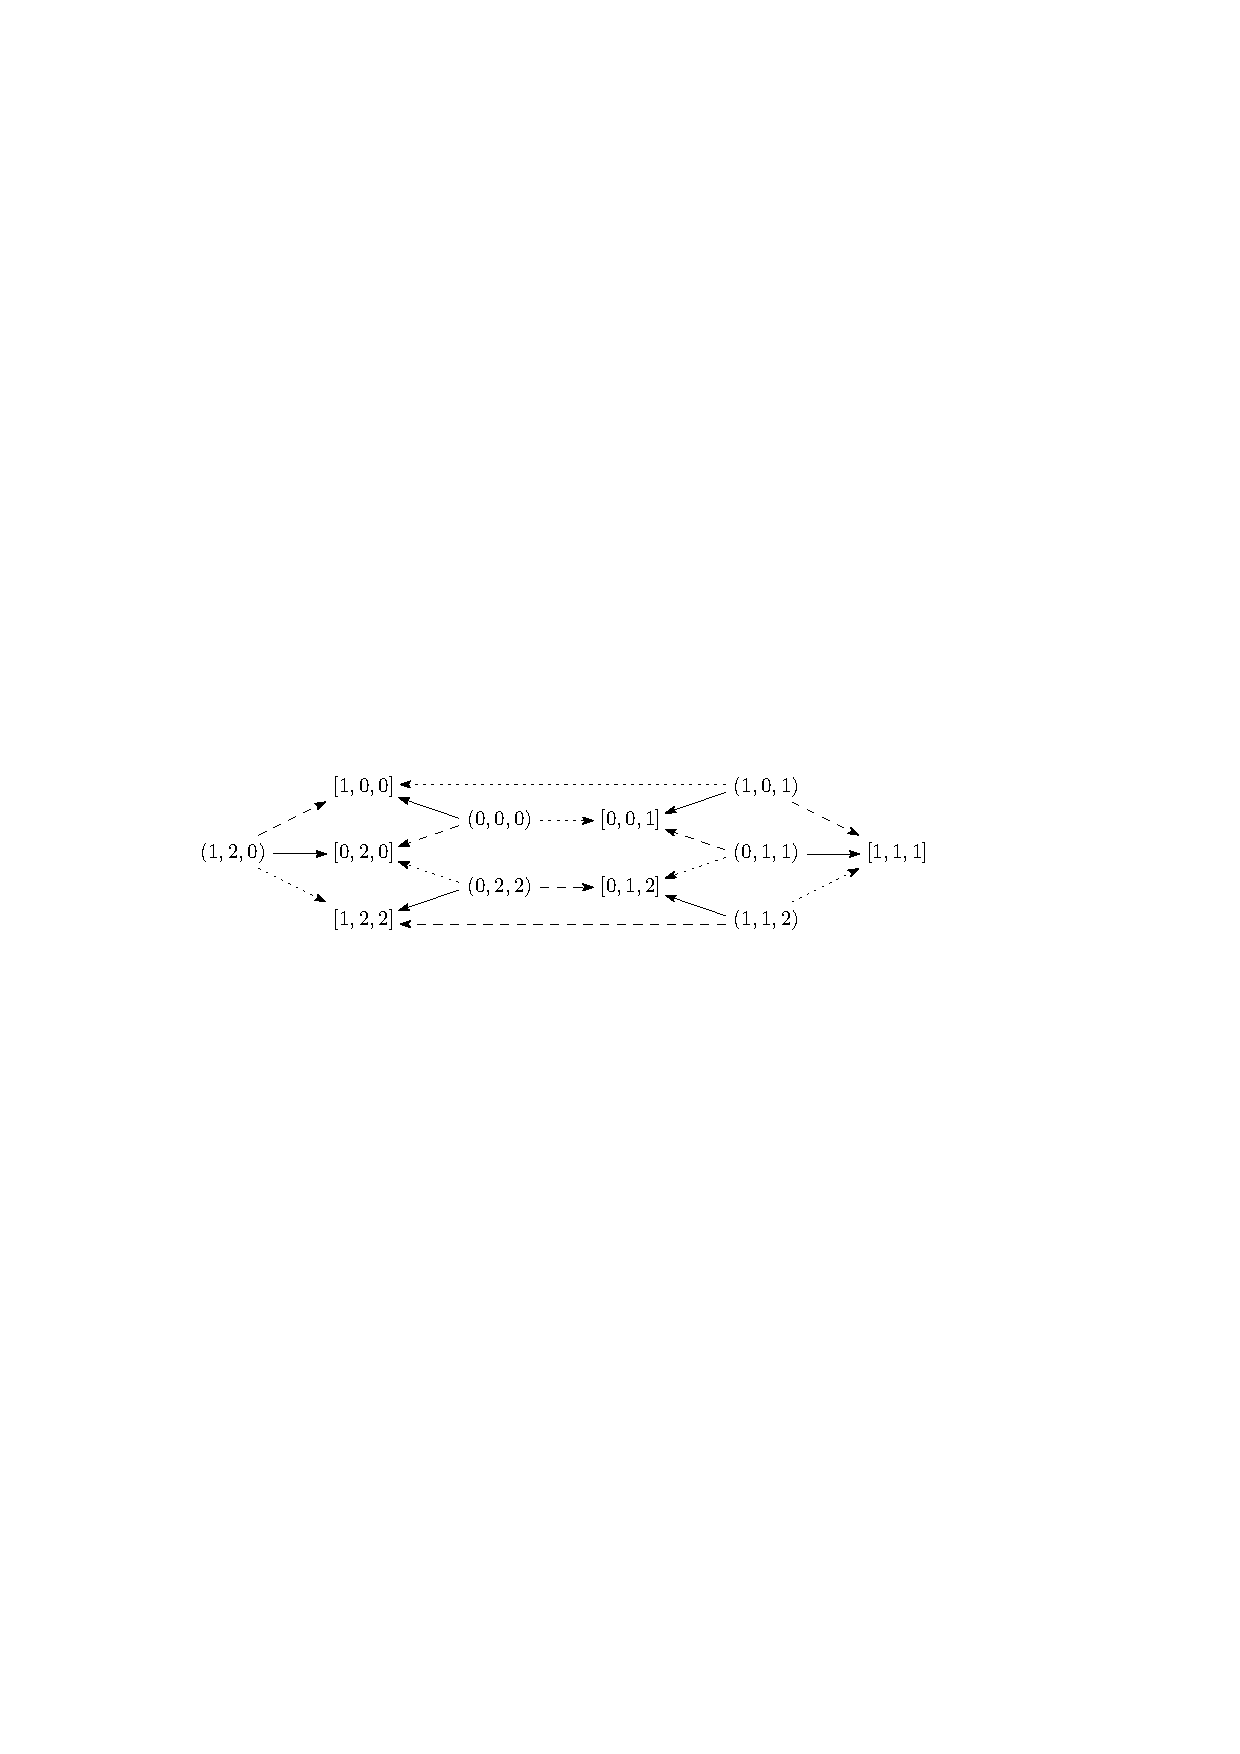
\includegraphics[width=0.9\textwidth]{img/graph_example.pdf}
\caption{Graph of a latin bitrade of size 6 on $\Z_2 \times \Z_3 \times \Z_3$.}
\label{fig:graph-bitrade}
\end{figure}
\end{exmp}%

\noindent
For later use, let us define maps $\sigma_R, \sigma_C, \sigma_S : T \cup T' \rightarrow T \cup T'$ by
\cosyalign{
 	\sigma_R(r,c,s) = (r',c,s) \mbox{ with } r \ne r',\\
 	\sigma_C(r,c,s) = (r,c',s) \mbox{ with } c \ne c', \\
 	\sigma_S(r,c,s) = (r,c,s') \mbox{ with } s \ne s'.
}%
The definition of the latin bitrade implies that these maps are involutions. They correspond to the edges of the graph -- on Figure \ref{fig:graph-bitrade},  $\sigma_R, \sigma_C, \sigma_S$ are represented by solid, dashed and dotted edges respectively.

\begin{lem}
\label{lem:connected-sigma}
A latin bitrade $(T,T')$ is connected if and only if for any $t_1,t_2 \in T \cup T'$ it is possible to get $t_2$ from $t_1$ by consequent application of $\sigma_R, \sigma_C, \sigma_S$.
\end{lem}
\begin{proof}
Simple, see the comment above.
\end{proof}

\begin{lem}
\label{lem:sigma-cycles}
Let $\{X,Y\} \subset \{R,C,S\}$. Then the mapping $\sigma_Y\sigma_X : T \cup T' \rightarrow T \cup T'$ is a permutation without a fixed point.
\end{lem}
\begin{proof}
The mapping is a bijection with inverse $\sigma_X\sigma_Y$ on a finite set, thus it is a permutation. It changes two coordinates of its argument, and therefore has no fixed points.
\end{proof}

Consider the following question: When is it possible to reconstruct a latin bitrade from its graph? Clearly we can do that only up to isotopy and conjugacy, as the graph representation forgets any orderings. Also, in every component of the graph we might switch roles of $T$ and $T'$.

The graph of a bitrade is edge 3-colorable. By excluding edges of one color, say corresponding to  R, the graph splits into cycles, in which all the elements have the same $R$-coordinate. If the $R$-coordinates in different cycles are different, the bitrade is called \emph{$R$-separated}. Analogously for $C$ and $S$.

\begin{defn}
 A latin bitrade is \emph{separated} if it is $R$-, $C$- and $S$-separated.
\end{defn}

Every latin bitrade can be transformed into a separated one -- for a symbol $x$ spanning multiple cycles, it suffices to introduce new symbols $x', x'', \dots$, one for each cycle, and relabel accordingly. Clearly, this new bitrade yields the same graph as the original one.

\begin{exmp}
The bitrade from Example \ref{exmp:graph-bitrade} is separated. Figure \ref{fig:separated-graph} illustrates the cycles after deletion of edges corresponding to $S$.

\begin{figure}[htb]
\centering
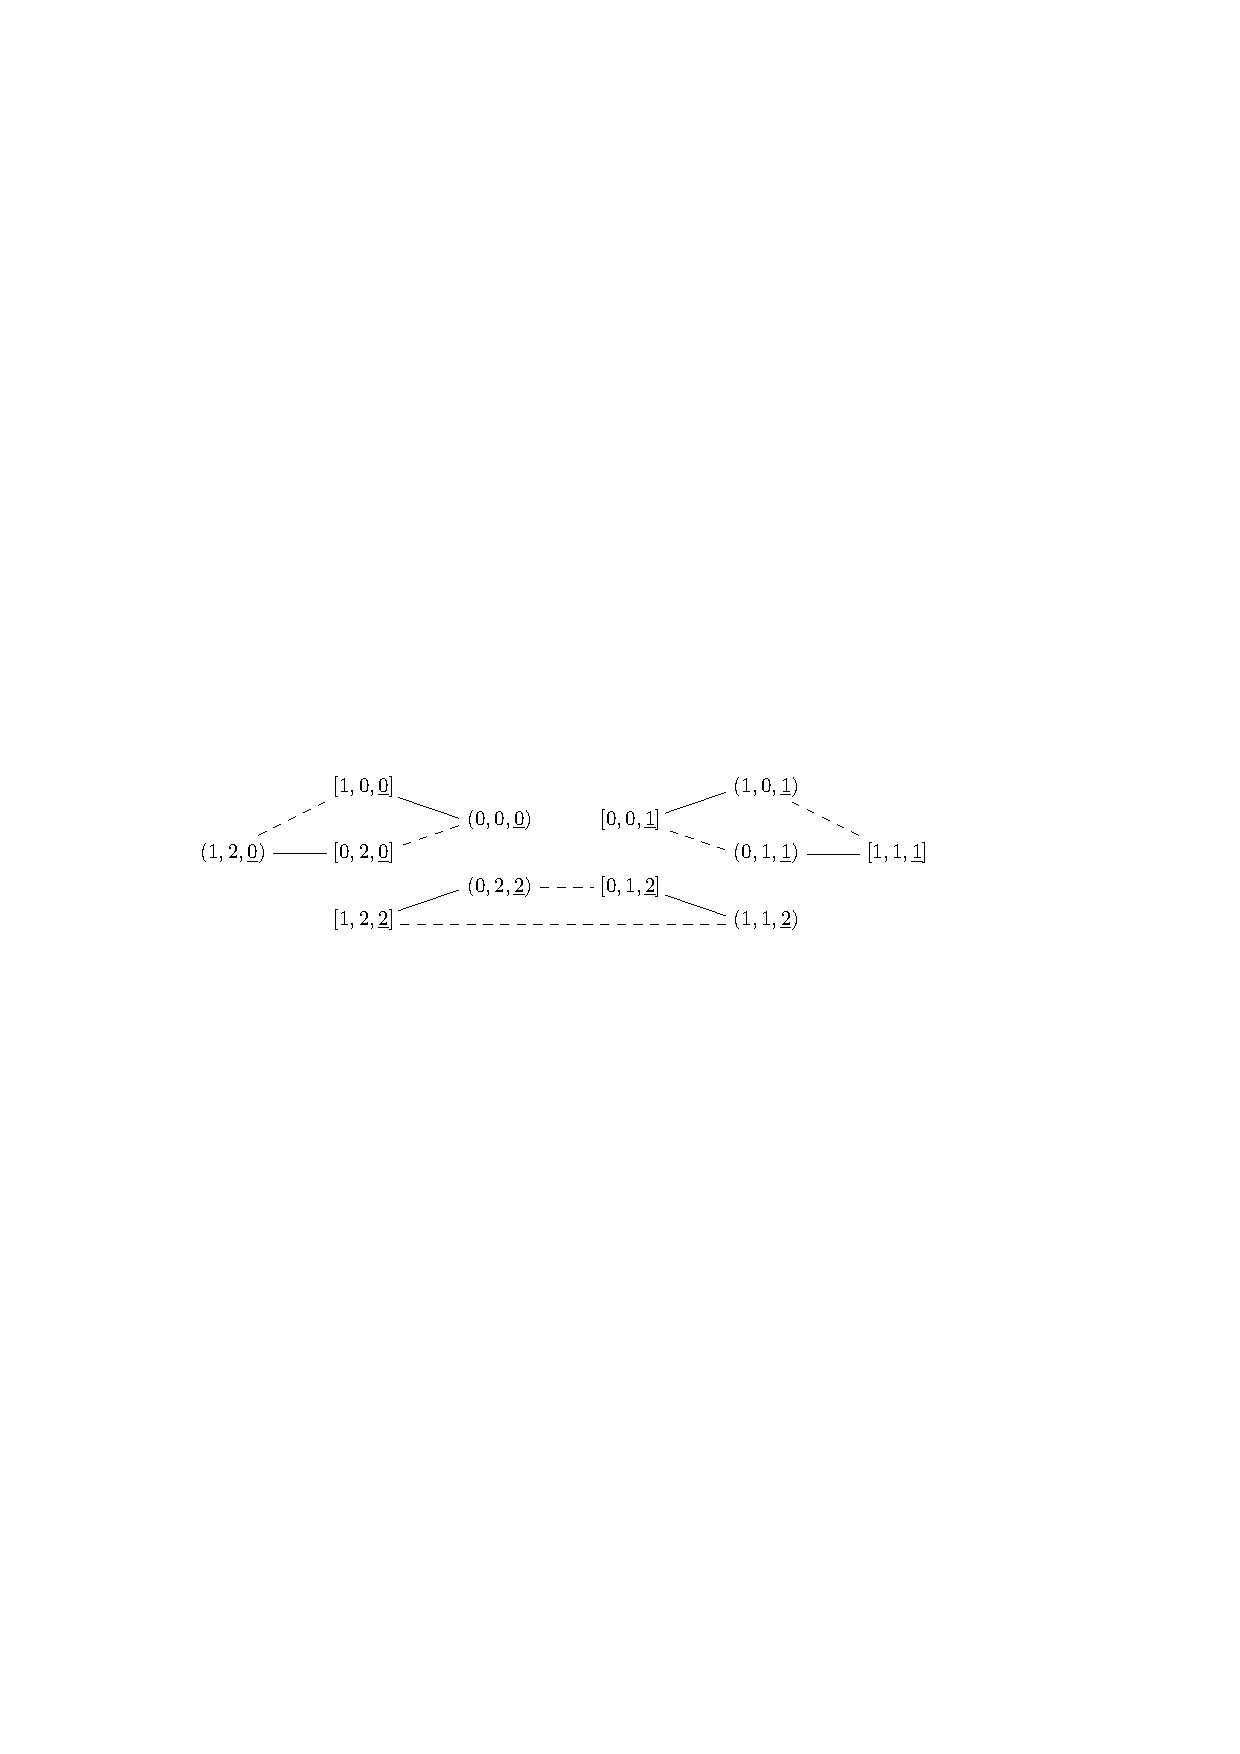
\includegraphics[width=0.9\textwidth]{img/separated.pdf}
\caption{2-color cycles in a separated latin bitrade.}
\label{fig:separated-graph}
\end{figure}
\end{exmp}%

%\begin{lem}
%\label{lem:3-coloring}
%Let $G$ be a planar cubic bipartite graph. Then there exists unique face 3-coloring of $G$.
%\end{lem}
%\begin{proof}
%This result was already known to Heawood. A proof of it can be found in \cite{Tutte48}.
%\end{proof}

The following results regarding the relation of a latin bitrade and its graph in the planar case are due to Cavenagh and Lisoněk \cite{CavenaghLisonek08}. We state them without a proof. They considered unordered latin squares $\{T,T'\}$. 

\begin{defn}
A graph is \emph{Eulerian} if each vertex is of even degree. \emph{A triangulation} of a plane is an embedding of a graph into the plane such that every face is a triangle.
\end{defn}

\begin{lem}
Dual of the graph of a connected spherical latin bitrade is an Eulerian triangulation.
\end{lem}
\begin{proof}
Trivial.
\end{proof}

\begin{thm}
\label{thm:connected-spherical-separated}
There is a bijection between the main classes of connected separated spherical unordered latin bitrades of size $v-2$ and the isomorphism classes of planar Eulerian triangulations on $v$ vertices.
\end{thm}%

\begin{cor}
\label{cor:connected-spherical-separated}
There is an algorithm to reconstruct a connected separated spherical latin bitrade $(T,T')$ from its graph up to isotopy, conjugacy, and switch of the roles of $T$ and $T'$.
\end{cor}%




\chapter{Embedding latin trades into groups}
\label{chap:lower-bound}

In this chapter we define $\gdist(n)$ and present a proof for the lower bound in Conjecture \ref{conj:main}. We proceed as Drápal and Kepka in \cite{DrapalKepka89} and \cite{DrapalKepka85}. Since their work is a bit older, they use old terminology and their proof seems to be difficult to understand. We attempted to redo the proof using modern terminology and make it more accessible.

Moreover, we were able to improve the constant in the lower bound from $e \approx 2.718$ to $3 \log_3(e) \approx 2.731$, which is the best constant known so far. The key part in doing so is Lemma \ref{lem:technical}.

There are other proofs of the lower bound available, but they are not as general as the one of Drápal and Kepka. The proof of Cavenagh and Wanless \cite{CavenaghWanless09} considers only planar latin bitrades and abelian groups. (On the other hand, it exhibits an interesting connection between determinants and permanents of certain matrices, which we omit.) Another proof by Cavenagh \cite{Cavenagh03} restricts itself to cyclic groups only.\footnote{The author suspects that the proof of Cavenagh is not complete -- he silently assumes that determinant of a certain matrix is nonzero, but the proof is missing.} The proof of Drápal and Kepka works with all latin bitrades and all finite groups.

%%%
%%%
%%%
\section{Sparse matrices}

\begin{defn}
A matrix is \emph{sparse} if its elements are from $\{0,1\}$ and there is at most one occurrence of 1 in every row.
\end{defn}

We denote by $\overbar{M}_r^c$ the matrix obtained from $M$ by excluding row $r$ and column~$c$.

\begin{lem}
\label{lem:sparse2}
Let $M_0,M_1$ be sparse matrices with the same number of rows such that $M = (M_0,M_1)$ is a square block matrix. Then $\det(M) \in \{-1,0,1\}$.
\end{lem}
\begin{proof}
Let $c_0,c_1$ be the number of columns in $M_0$ and $M_1$ respectively. The proof is by induction on $n := c_0+c_1$. The case with $n=1$ is trivial. Therefore assume $n>1$.

There are at most two ones in every row of M.
\begin{cosyitemize}
	\item If there is a row with zeros only, then $\det(M) = 0$.
	\item If every row contains exactly two ones, then
		\begin{cosyeqnarray}
			v := (\underbrace{1,\dots,1}_{c_0},\underbrace{-1,\dots,-1}_{c_1}) \nonumber
		\end{cosyeqnarray}%
		is such that $Mv^T = 0$. Thus $M$ is singular and $\det(M) = 0$.
	\item Otherwise there is a row $r$ which contains only a single one in column $c$. Then expanding the determinant by row $r$ yields
	 \begin{cosyeqnarray}
	 	\det(M) = \pm \det(\overbar{M}_r^c).
	 \end{cosyeqnarray}%
	The matrix $\overbar{M}_r^c$ consists also from two sparse matrices, thus the result follows by induction.
\end{cosyitemize}
\end{proof}

\begin{lem}
\label{lem:sparse3}
Let $M_0,M_1,M_2$ be sparse matrices of sizes $n \times c_0, n \times c_1, n \times c_2$ such that $M = (M_0,M_1,M_2)$ is a square block matrix. Let $k_i$ denote the number of ones in column $i$. Then
\begin{cosyeqnarray}
	|\det(M)| \leq \prod_{i \in [c_0]} k_i.
\end{cosyeqnarray}%
\end{lem}
\begin{proof}
The proof is by induction on $c_0$. Denote $M = (m_{i,j})_{i,j \in[n]}$.
\begin{enumerate}
	\item If $c_0 = 0$, then $|\det(M)| \leq \prod_{i=0}^{0} k_i = 1$ holds by Lemma \ref{lem:sparse2}.
	\item Otherwise expand by the first column:
	\begin{cosyeqnarray}
		|\det(M)| \leq \sum_{i\in[n]} m_{i,0}\,|\det(\overbar{M}_i^1)| \leq k_0 \prod_{i \in [1, c_0)} k_i.
	\end{cosyeqnarray}%
	The last inequality holds since there are $k_0$ nonzero summands and the product majorizes each subdeterminant from induction.
\end{enumerate}
\end{proof}

For our final result we need the following technical lemma:

\begin{lem}
\label{lem:technical}
Let $n$ be a positive integer and $k_0 + \dots + k_{m-1} = n$ for an integer $m$. Then
\begin{cosyeqnarray}
	\prod_{i \in [m]} k_i \leq 3^{n/3}.
\end{cosyeqnarray}%
\end{lem}
\begin{proof}
For $n=1$ it holds trivially, let us assume $n > 1$. Let $k_0 \leq \dots \leq k_{m-1}$ be lexicographically smallest such that the maximum is attained. Observe:
\begin{cosyitemize}
	\item $2 \cdot (k-2) \geq k$ for $k \geq 4$, therefore $k_i \leq 3$;
	\item $(1+k) > 1 \cdot k$, therefore $k_i > 1$;
	\item $3 \cdot 3 > 2 \cdot 2 \cdot 2$, therefore there are at most two twos amongst $k_i$.
\end{cosyitemize}%
Thus there are 3 possibilities:
\cosyalig{
&n =3k &\Rightarrow&\ k_0 = \dots = k_{m-1} = 3 &\Rightarrow& \prod k_i = 3^{n/3} \\
&n =3k+2 &\Rightarrow&\ k_0 = 2, k_1 = \dots = k_{m-1} = 3 &\Rightarrow& \prod k_i = 2\cdot3^{(n-2)/3} \\
&n =3k+4 &\Rightarrow&\ k_0 = k_1 = 2, k_2 = \dots = k_{m-1} = 3 &\Rightarrow& \prod k_i = 4\cdot3^{(n-4)/3} 
}
Where the products are over $i \in [m]$. Each of them is less than or equal to $3^{n/3}$, thus we are done.
\end{proof}

\begin{lem}
\label{lem:3-block-sparse-det}
Let $M_0,M_1,M_2$ be sparse matrices such that $M = (M_0,M_1,M_2)$ is a  square block $n \times n$ matrix. Then
\begin{cosyeqnarray}
 	|\det(M)| \leq 3^{n/3}
\end{cosyeqnarray}% 
and thus $3 \log_3(|\det(M)|) \leq n$.
\end{lem}
\begin{proof}
Let $c_0$ be the number of columns of $M_0$ and $k_i$ the number of ones in the column $i$. Since $M_0$ is sparse, surely $\sum_{i \in [c_0]} k_i \leq n$. The proof is finished by combining Lemmas \ref{lem:sparse3} and \ref{lem:technical}:
\begin{cosyeqnarray}
	|\det(M)| \leq \prod_{i \in [c_0]} k_i \leq 3^{n/3}.
\end{cosyeqnarray}%
\end{proof}

%%%
%%%
%%%
\section{Trade matrix}
Recall that
\begin{itemize}
	\item $R = \{r_0,\dots,r_{|R|-1}\}$ denotes the set of rows,
	\item $C = \{c_0,\dots,c_{|C|-1}\}$ denotes the set of columns and
	\item $S = \{s_0,\dots,s_{|S|-1}\}$ denotes the set of symbols.
\end{itemize}
Without loss of generality assume that these sets are disjoint and let $X = R \cup C \cup S$.

\begin{defn}
Let $T$ be a latin trade. We define a matrix $M = (m_{i,j})$ of size $|T| \times |X|$ such that if we index the rows by elements of $T$ and columns by elements of $X$, then
\begin{cosyeqnarray}
	t = (r,c,s) \in T \Rightarrow
	\begin{cases}
		m_{t,r} = m_{t,c} = m_{t,s} = 1, & \\
		m_{t,x} = 0 & \textrm{ for } x \in X \setminus \{r,c,s\}.
	\end{cases}
\end{cosyeqnarray}%
\end{defn}
We call it the \emph{trade matrix} and denote by $M_T$.

\begin{lem}
Suppose that all elements of $X$ are used in a connected latin trade $T$. Then
\cosyalign{
	\Ker M_T = \{(\underbrace{x, \dots, x}_{|R|}, \underbrace{y, \dots, y}_{|C|}, \underbrace{z, \dots, z}_{|S|}) \mid x+y+z = 0\} \label{eq:KerMT}
}%
where $M_T$ is considered as a matrix over $\Q$.
\end{lem}
\begin{proof}
The proof is divided into several steps.

%
%
\item \textbf{Step 1.}
Denote the set in (\ref{eq:KerMT}) by $V$. Any vector $v \in V$ is surely a solution for $M_Tv^T = 0$. Let $f:X \rightarrow \Q$ be defined by
\begin{align}
	v = (f(r_0), \dots, f(c_0), \dots, f(s_0), \dots).
\end{align}
Choose $(x_0, y_0, z_0) \in T$ such that $f(z_0)$ is maximal. By resetting
\begin{align}
	v := v+(-f(x_0), \dots, -f(y_0), \dots,f(x_0)+f(y_0), \dots)
\end{align}
we obtain a solution in which $f(x_0) = f(y_0) = f(z_0) = 0$. Now it suffices to prove that $f(x) = 0$ for any $x \in X$. To shorten notation, we denote $f(x,y,z) = f((x,y,z)) = (f(x),f(y),f(z))$.

%
%
\item \textbf{Step 2.}
For all $(x,y,z) \in T$ holds $f(x)+f(y)+f(z)=0$. Since $0$ is the largest element of $\{f(z) \mid z \in S\}$ and $T'$ occupies the same cells as $T$, for all $(x,y,z) \in T \cup T'$
\begin{align}
	f(x) + f(y) \geq 0.
\end{align}
In steps 3 and 4 we prove that if $t \in T\cup T'$ and $f(t) = (0,0,0)$, then
\begin{align}
	f(\sigma_Y(t)) = (0,0,0)
\end{align}
for $Y \in \{R, C, S\}$. Since the bitrade is connected, Lemma \ref{lem:connected-sigma} implies that $f(t) = (0,0,0)$ for all $t \in T \cup T'$. Because all symbols are used in the bitrade, from that we have the desired $f(x) = 0$ for all $x \in X$.

%
%
\item \textbf{Step 3.}
Let $(x,y,z) \in T'$ such that $f(x,y,z) = (0,0,0)$. Then
\begin{align}
	f(\sigma_R(x,y,z)) = f(x',y,z) = (f(x'), 0, 0)
\end{align}
for some $x' \in R$ such that $(x',y,z) \in T$. Therefore $f(x') + 0 + 0 = 0$. Similarly for $\sigma_C$ and $\sigma_S$.

%
%
\item \textbf{Step 4.}
Now let $(x_0,y_0,z) \in T$ such that $f(x_0,y_0,z)=(0,0,0)$. Consider a chain of elements in $T \cup T'$:
\begin{align*}
	(x_0,y_0,z) &\in T &\xrightarrow{\sigma_C}& &(x_0,y_1,z) &\in T' & \xrightarrow{\sigma_R} \\
	(x_1,y_1,z) &\in T &\xrightarrow{\sigma_C}& &(x_1,y_2,z) &\in T' & \xrightarrow{\sigma_R} \\
	(x_2,y_2,z) &\in T &\xrightarrow{\sigma_C}& &(x_2,y_3,z) &\in T' & \dots
\end{align*}
From the inequality we have
\begin{align*}
	f(x_0) + f(y_0) &= 0, \quad f(x_0) + f(y_1) \geq 0, \\
	f(x_1) + f(y_1) &= 0, \quad f(x_1) + f(y_2) \geq 0, \\
	f(x_2) + f(y_2) &= 0, \quad f(x_2) + f(y_3) \geq 0,\ \dots, 
\end{align*}
which yields
\begin{align*}
	0 &= f(x_0) \leq f(x_1) \leq f(x_2) \leq \dots \\
	0 &= f(y_0) \geq f(y_1) \geq f(y_2) \geq \dots
\end{align*}
According to Lemma \ref{lem:sigma-cycles}, the chain is a non-trivial cycle, and thus all terms in the inequalities equal to zero. Especially $f(\sigma_C(x_0,y_0,z)) = (0,0,0)$.

The result for $\sigma_R$ can be obtained by changing the roles of $\sigma_R$ and $\sigma_C$.

For $\sigma_S$, consider a cycle generated by alternating $\sigma_C$ and $\sigma_S$. We already know that $f(\sigma_S\sigma_C(x_0,y_0,z)) = \sigma_S(0,0,0) = (0,0,0)$. Therefore all elements in the cycle are mapped to $(0,0,0)$. By reversing the cycle we get the result.

\end{proof}

\begin{cor}
\label{cor:rank-mt}
Suppose that all elements of $X$ are used in a connected latin trade $T$. Then the trade matrix $M_T$ has rank $|X|-2$ over $\Q$.
\end{cor}

\begin{note}
Suppose that $M$ is a submatrix of $M_T$ of rank $|X|-2$. It must have been obtained from $M$ by deleting two columns and some rows. These two columns cannot be both from $R$. If they were, then
\cosyalign{
	(\underbrace{0, \dots, 0}_{|R|-2}, \underbrace{y, \dots, y}_{|C|}, \underbrace{-y, \dots, -y}_{|S|})
}%
would be solutions of $Mv^T = 0$, which contradicts the regularity of $M$. Therefore the deleted columns must be from two different sets from $R$, $C$, $S$.
\end{note}


\begin{cor}
\label{cor:size-of-t}
$|T| \geq |X|-2$.
\end{cor}

%%%
%%%
%%%
\section{Homotopies from latin trades to groups}

\begin{defn}
\emph{A Cayley table} of a group $G$ is a latin square $L \subset G \times G \times G$ such that $(r,c,s) \in L$ if and only if $r \cdot c = s$. We denote it by $G$ when no confusion can arise.
\end{defn}

For abelian groups, we will use different definition:

\begin{defn}
\emph{A Cayley table} of an abelian group $(G,+)$ is a latin square $L \subset G \times G \times G$ such that $(r,c,s) \in L$ if and only if $r + c + s = 0$.
\end{defn}

It easily follows that the Cayley tables by first and second definition are isotopic. Because we will be interested in existence of homotopies into Cayley tables, it does not matter which definition we use.

\begin{defn}
Let $z(G)$ denote the size of the smallest trade $T$ such that there exist a non-trivial homotopy from $T$ to $G$. Let \emph{$z(n)$} be the minimum across all groups of order $n$.
\end{defn}

\begin{lem}
\label{lem:p-leq-det}
Let $p$ be a prime, $T$ a connected latin trade using all symbols in $X$, $h: T \rightarrow \Z_p$ a non-trivial homotopy and $M$ any submatrix of $M_T$ of rank $|X-2|$. Then $p \leq \det(M)$.
\end{lem}
\begin{proof}
Let $h = (h_R,h_C,h_S)$. Then
\begin{align*}
	v = \big(\underbrace{h_R(r_0), \dots, h_R(r_{|R|-1})}_{|R|},\underbrace{h_C(c_0), \dots, h_C(c_{|C|-1})}_{|C|}, \underbrace{h_S(s_0), \dots, h_S(s_{|S|-1})}_{|S|}\big)
\end{align*}
is a solution of $M_Tv^T = 0$ over $\Z_p$. Without loss of generality assume that columns $r_0$, $c_0$ were deleted from $M_T$ to obtain $M$ (see note after Corollary \ref{cor:rank-mt}). Also suppose that $h_R(r_0) = 0 = h_C(c_0)$, otherwise we can set
\cosyalig{
	h_R' := h_R - h_R(r_0), \quad h_C' := h_C - h_C(c_0), \quad	h_S' := h_S + h_R(r_0) + h_C(c_0).
}%
Then
\begin{align*}
	w = \big(\underbrace{h_R(r_1), \dots, h_R(r_{|R|-1})}_{|R|-1},\underbrace{h_C(c_1), \dots, h_C(c_{|C|-1})}_{|C|-1}, \underbrace{h_S(s_0), \dots, h_S(s_{|S|-1})}_{|S|}\big)
\end{align*}
is a solution of $Mw^T = 0$ over $\Z_p$ which is non-trivial, since $h$ is non-trivial.

Therefore $\det(M) = 0$ in $\Z_p$, which means $p \mid \det(M)$.
\end{proof}

\begin{lem}
\label{lem:lower-bound-zp}
$3 \log_3(p) \leq z(p)$.
\end{lem}%
\begin{proof}
Let $T$ be a latin trade such that $|T| = z(p)$ and there exists a non-trivial homotopy $T \rightarrow \Z_p$. From Lemma \ref{lem:p-leq-det} we know that $p \leq \det(M)$ for a submatrix of $M_T$ of rank $|X|-2$.

We can write $M_T = (M_0, M_1, M_2)$ for sparse matrices $M_0$, $M_1$, $M_2$, and therefore any submatrix $M$ of $M_T$ is of the same type. Thus from Lemma \ref{lem:3-block-sparse-det} and Corollary \ref{cor:size-of-t}
\cosyalign{
	p \leq \det(M) \leq 3^{(|X|-2)/3} \leq 3^{z(p)/3}.
}%
\end{proof}

\begin{lem}
\label{lem:nontrivial-homotopy-normal-subgroup}
Let $H$ be a normal subgroup of $G$ and $h: T \rightarrow G$ is a non-trivial homotopy. Then there exists a non-trivial homotopy $h_0: T \rightarrow H$ or $h_1: T \rightarrow G/H$.
\end{lem}
\begin{proof}
Let $\pi: G \times G \times G \rightarrow G/H \times G/H \times G/H$ is the natural projection. If $h_1 := \pi h$ is non-trivial, we are done. Otherwise $\Img(h) \subset H \times H \times H$ and we can set $h_0 := h$.
\end{proof}

\begin{lem}
\label{lem:zG-is-zp}
Let $G$ be a group of odd order. Then
\cosyalign{
	z(G) = \min \{z(p) \mid \mbox{ prime $p$ divides $|G|$} \}.
}%
\end{lem}
\begin{proof}
Lemma \ref{lem:nontrivial-homotopy-normal-subgroup} together with odd order theorem imply the "$\geq$" inequality. The other one is implied by Cauchy's theorem.
\end{proof}

%%%
%%%
%%%
\section{Lower bound for gdist(n)}

\begin{defn}
A latin trade $T$ \emph{can be embedded} (or \emph{is embeddable}) in a group $G$ if there exists an injective homotopy from $T$ to $G$.

Let \emph{$\gdist(G)$} denote the size of the smallest trade embeddable in $G$ and let \emph{$\gdist(n)$} be the minimum across all groups of order $n$.
\end{defn}

From the tabular point of view, a latin trade $T$ can be embedded in a group $G$ if we can find an isotopic copy of the partial latin square $T$ inside of the Cayley table of $G$. The next lemma states that $\gdist(G)$ is the smallest number of cells in the Cayley table of $G$ that have to be changed in order to get another latin square:

\begin{lem}
Let $G$ be a group. Then
\cosyalign{
	\gdist(G) = \min \{|G \setminus L| : L \subset G \times G \times G \mbox{ is a latin square}, L \ne G \}.
}%
\end{lem}
\begin{proof}
$(G \setminus L, L \setminus G)$ is a latin bitrade, hence "$\leq$" holds. On the other hand, if $(T,T')$ is a latin bitrade embeddable in $G$ via injective homotopy $h$, then $G \setminus h(T) \cup h(T')$ is a latin square.
\end{proof}

\begin{exmp}
See Figure \ref{fig:z5-embedded-trade}.
\end{exmp}%

\begin{figure}[htb]
	\centering
	\begin{minipage}{.35\linewidth}
		\begin{center}
		\begin{tabular}{| c c c c |}
			\hline
				0 &   & 3 & 4 \\
				  & 3 & 4 & 0 \\
				3 & 0 &   &   \\
			\hline
		\end{tabular} \\
		\bigskip
		$T$
		\end{center}
	\end{minipage}
	\begin{minipage}{.35\linewidth}
		\begin{center}
		\begin{tabular}{| c c c c |}
			\hline
				3 &   & 4 & 0 \\
				  & 0 & 3 & 4 \\
				0 & 3 &   &   \\
			\hline
		\end{tabular}\\
		\bigskip
		$T'$
		\end{center}
	\end{minipage}\\
	\bigskip%
	\begin{minipage}{.35\linewidth}
		\begin{center}
		\begin{tabular}{| c c c c c |}
			\hline
				\M0 & 1 & 2   & \M3 & \M4 \\
				1   & 2 & \M3 & \M4 & \M0 \\
				2   & 3 & 4   & 0   & 1   \\
				\M3 & 4 & \M0 & 1   & 2   \\
				4   & 0 & 1   & 2   & 3   \\
			\hline
		\end{tabular}\\
		\bigskip
		$\Z_5$
		\end{center}
	\end{minipage}
	\begin{minipage}{.35\linewidth}
		\begin{center}
		\begin{tabular}{| c c c c c |}
			\hline
				\M3 & 1 & 2   & \M4 & \M0 \\
				1   & 2 & \M0 & \M3 & \M4 \\
				2   & 3 & 4   & 0   & 1   \\
				\M0 & 4 & \M3 & 1   & 2   \\
				4   & 0 & 1   & 2   & 3   \\
			\hline
		\end{tabular}\\
		\bigskip
		$L$
		\end{center}
	\end{minipage}
	\caption{Latin trade $T$ embedded in $\Z_5$ and the corresponding latin square $L$.}
	\label{fig:z5-embedded-trade}
\end{figure}

\begin{thm}
\label{thm:lower-bound}
Let $p$ be the smallest prime factor of $n \geq 2$. Then
\cosyalign{
	3\log_3(p) \leq \gdist(n).
}%
\end{thm}%
\begin{proof}
If $n$ is even, then $p=2$, $\gdist(n) = 4$ and the inequality holds. Otherwise by Lemmas \ref{lem:lower-bound-zp} and \ref{lem:zG-is-zp} there is a prime factor $p_0$ of $|G|$ such that
\begin{align}
	3 \log_3(p_0) \leq z(p_0) = z(G) \leq \gdist(G),
\end{align}
where the last inequality is trivial from definition. The fact that $p \leq p_0$ finishes the proof.
\end{proof}

\chapter{Dissections of equilateral triangles}
\label{chap:dissections}

The study of dissections was initiated by the paper \emph{The dissection of rectangles into squares} by Brooks, Smith, Stone and Tutte \cite{BrooksSmithStoneTutte40}. They answered the question whether it is possible to dissect a square into some number of unequal squares (yes, it is), and developed methods to study such dissections.\footnote{They showed, for example, that dissections into squares are related to electrical circuits obeying Kirchhoff's laws.}

Inspired by a puzzle called \emph{Mrs Perkins's quilt} by Dudeney~\cite{Dudeney17}, Conway~\cite{Conway64} considered the case where the dissecting squares can be equally large. He proposed a question about the minimal number of integer-sided squares needed to dissect a square of side $n$. It is easy to observe that when $n$ is divisible by an integer $d \geq 2$, then it is possible to use a scaled up dissection of a square of side $d$. Therefore he considered only dissections where the dissecting squares do not have a common factor.

Conway proved that at least $c \log(n)$ squares are needed. A year later Trustrum \cite{Trustrum65} proved that $O(\log(n))$ is sufficient, and thus established that the answer is asymptotically logarithmic. However, the best constants in the estimates do not appear to be known.

\bigskip

In this chapter we prove that it is possible to dissect an equilateral triangle of side $n$ into $O(\log(n))$ equilateral triangles. We do so by modifying a dissection of a rectangle into squares. We explain the connection to latin bitrades and prove the upper bound in Conjecture \ref{conj:main}. The last section of this chapter contains a generalization of the dissection method, which might be useful for further improvements of the upper bound.

\bigskip

\noindent\hspace{1em}
Note that the first one to study dissections of equilateral triangles was Tutte~\cite{Tutte48}. 


%%%
%%%
%%%
\section{Definitions}

Unless specified otherwise, from now on we use \emph{triangle} instead of \emph{equilateral triangle} for brevity.

\begin{defn}
\emph{A dissection of size $m$ of a rectangle} is a set of $m$ squares of integral side which cover the rectangle and overlap at most on their boundaries. Such a dissection is \emph{$\oplus$-free} if no four squares share a common point, it is \emph{prime} if their sides do not have a common factor.

We denote by $r_d(n)$ the minimal size of a dissection of an $n \times (n+d)$ rectangle.
\end{defn}

\begin{defn}
\label{defn:triangle-dissection}
\emph{A dissection of size $m$ of a triangle} is a set of $m$ triangles of integral side which cover the original triangle and overlap at most on their boundaries. Such a dissection is \emph{$\circledast$-free} if no six triangles share a common point, \emph{prime} if their sides do not have a common factor, and \emph{trivial} if $m=1$.

We denote by $t(n)$ (respectively, $\hat t(n)$) the minimal size of a non-trivial dissection (respectively, prime dissection) of a triangle of side $n$.
\end{defn}

We use terms \emph{dissection} and \emph{tiling} interchangeably. Also by \emph{rectangle} or \emph{triangle dissection} we mean \emph{dissection of a rectangle} or \emph{triangle} respectively. Moreover, for squares and triangles we mean the same by \emph{side} and \emph{size}.

Note that only 2, 3, 4 or 6 triangles can share a common point in a triangle dissection. Therefore $\circledast$-freeness implies that actually no more than 4 triangles meet at one point.

\begin{lem}
For a positive integer $n$ and a prime $p$ holds $t(n) \leq \hat t(n)$ and $t(p) = \hat t(p)$.
\end{lem}
\begin{proof}
Trivial.
\end{proof}

%%%
%%%
%%%
\section{Logarithmic dissection of a rectangle}
\label{sec:log-rectangle}

Let us describe an algorithm to dissect an $n \times (n+3)$ rectangle for $n \geq 2$. Fix the orientation of the rectangle with the shorter side on the left. For convenience, we say that a dissection is \emph{padded} if it has a square of side at least 2 in the upper left corner. Then the algorithm is as follows:

\begin{alg} \ 
\begin{enumerate}
		\item[(A1)] For $n=2,3,4,5,6,7,8,9,10$ dissect into $4,2,5,5,3,6,6,4,7$ squares respectively such that the dissection is $\oplus$-free and padded;
		\item[(A2)] for $n$ of form $4k+z$ with $k \geq 2, z \in \{3,4,5,6\}$, depending on $z$ dissect into $3$ or $5$ squares and a rectangle of size $2k \times 2(k+3)$. Then dissect this rectangle with two times larger tiles recursively. Figure \ref{fig:kk3} illustrates the method.
	\end{enumerate}
\end{alg}%
	
\begin{figure}[htb]
\centering
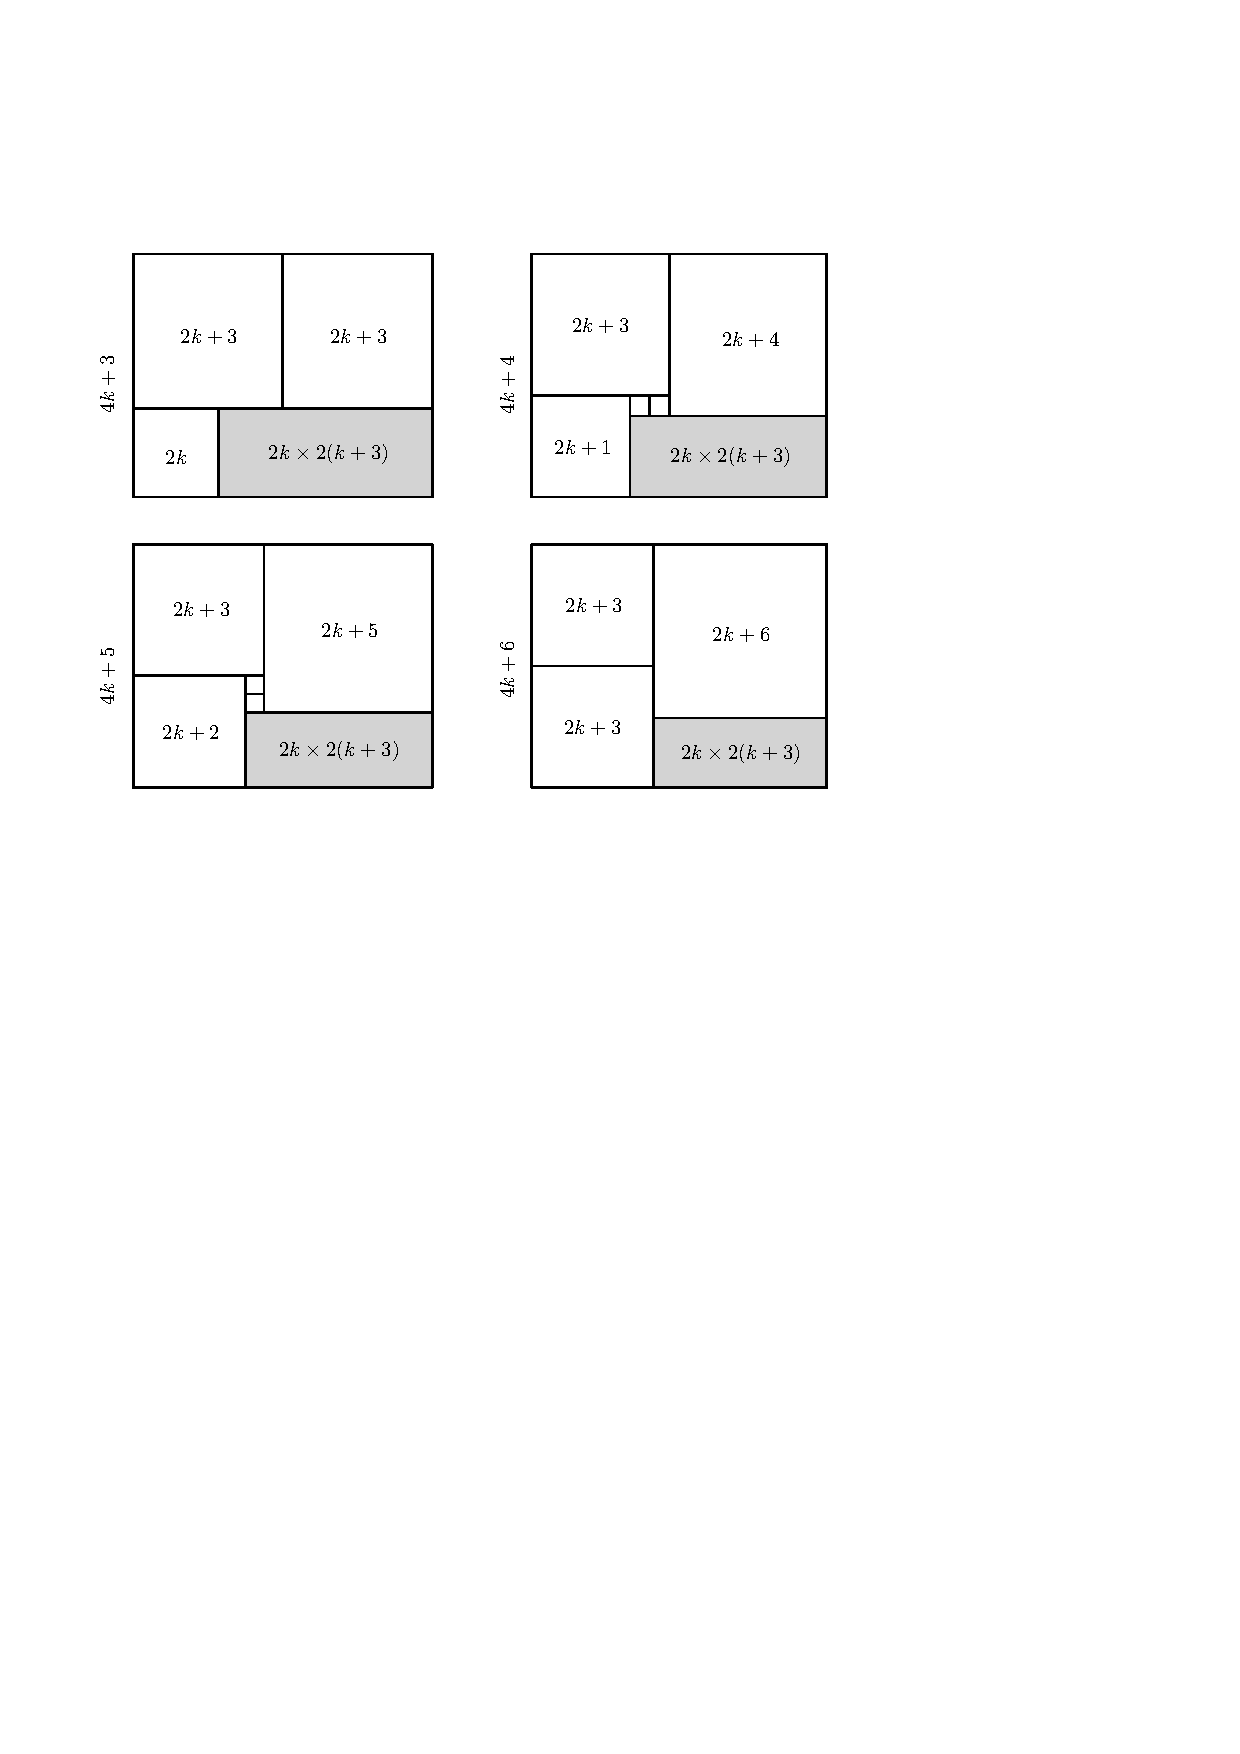
\includegraphics[width=0.9\textwidth]{img/kk3.pdf}
\caption{Dissecting a rectangle of size $n \times (n+3)$}
\label{fig:kk3}
\end{figure}


Recall that by $r_3(n)$ we denote the smallest size of a $\oplus$-free dissection of an $n \times (n+3)$ rectangle. Note that $r_3(1) = 4$, and let us estimate the remaining values using the algorithm:

\begin{lem}
\label{lem:r3n}
Let $n \geq 2$ be an integer. Then the algorithm results in a padded $\oplus$-free dissection of an $n \times (n+3)$ rectangle. Furthermore $r_3(n) \leq 5\log_4(n)+\frac{3}{2}$.
\end{lem}
\begin{proof}
The proof is by induction on $n$; for $n$ in (A1) the claim holds.

Let $n = 4k+z$ where $k \geq 2, z \in \{3,4,5,6\}$. By (A2) we clearly get a padded rectangle dissection. The inside of the recursively dissected rectangle $2k \times 2(k+3)$ is $\oplus$-free by the induction hypothesis, and the outside is such by design. Therefore the only points where $\oplus$-freeness might be broken lie on its border.

However, the recursive dissection is padded and tiled with two times larger tiles, therefore there is a square of size at least 4 in the upper left corner which covers all possible problematic points.

Finally,
\begin{cosyeqnarray}
	r_3(4k+z) \leq 5 + r_3(k) \leq 5 + 5\log_4(k) + \tfrac{3}{2} \leq 5 \log_4(4k+z) + \tfrac{3}{2}.
\end{cosyeqnarray}%
\end{proof}

%%%
%%%
%%%
\section{Logarithmic dissection of a triangle}
\label{sec:log-dissection-triangle}

\begin{lem}
\label{lem:triangles-to-squares}
Let $5 \leq n = 2k+3$ be an odd integer not divisible by 3. Then $\hat t(n) \leq 2\,r_3(k)+2$.
\end{lem}

\begin{proof}
Consider a triangle of side $n$. We can cut off triangles of sides $k$ and $(k+3)$ from two of its corners, which leaves us with a parallelogram of sides $k$ and $(k+3)$. By a linear mapping $f$ we can transform it into a $k\times (k+3)$ rectangle (see Figure \ref{fig:transf}), which can be dissected into $r_3(k)$ squares.

\begin{figure}[htb]
\centering
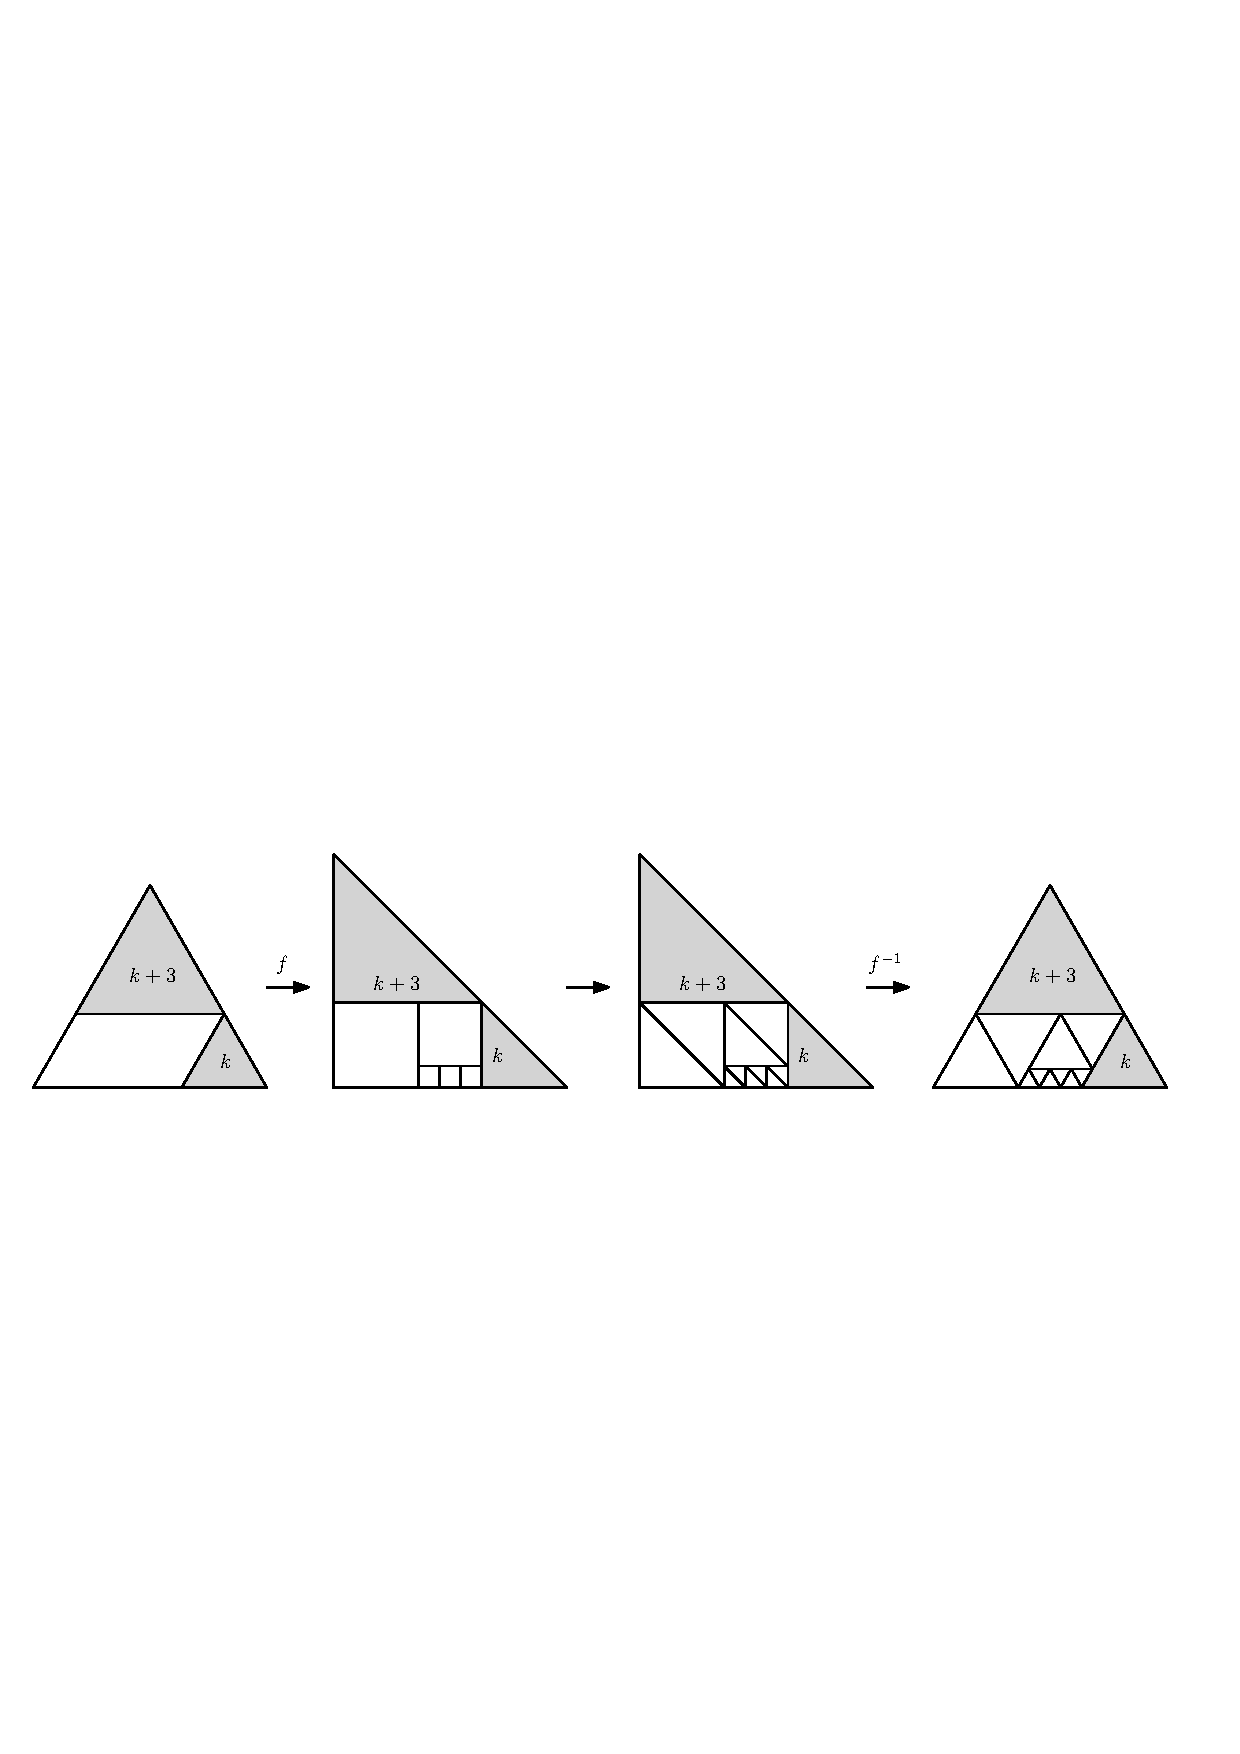
\includegraphics[width=0.9\textwidth]{img/transf.pdf}
\caption{Dissecting a triangle using a dissection of a rectangle.}
\label{fig:transf}
\end{figure}

Now, every square in the dissection can be diagonally cut into two right-angled triangles, such that after application of $f^{-1}$ they transform into equilateral triangles. This gives us a dissection of the original triangle into $2\,r_3(k)+2$ triangles. Moreover $\gcd(k+3,3) =\gcd (k,3)$ and $3 \nmid k$, therefore the dissection is prime.

It remains to prove $\circledast$-freeness. Clearly, the condition cannot be violated on the sides of the parallelogram.

Note that all the diagonal cuts have to be parallel, which means that there is at most one of them adjacent to every square corner (the rectangle dissection is $\oplus$-free). Thus we increase the number of shapes incident with every point at most by one and the resulting dissection is $\circledast$-free.
\end{proof}

\begin{cor}
\label{cor:hat-t-odd-n}
Let $n > 1$ be an odd integer not divisible by 3. Then $\hat t(n) < 5\log_2(n)$.
\end{cor}
\begin{proof}
The conditions imply $n \geq 5$. Now by plugging $k = \frac{n-3}{2}$ into Lemma~\ref{lem:r3n}:
\cosyalign{
	\hat t(n) \leq 2r_3(\tfrac{n-3}{2})+2 \leq 10 \log_4(\tfrac{n-3}{2}) + 5 = 5 \log_2(n-3) < 5 \log_2(n).
}
\end{proof}


\begin{thm}
\label{thm:t-log-bound}
Let $n \geq 2$ be an integer. Then $\hat t(n) < 5\log_2(n)$.
\end{thm}
\begin{proof}

Set $n = 2^p3^qr$, where $p,q,r$ are nonnegative integers such that $\gcd(r,6) = 1$. Use the following algorithm to get a dissection of a triangle of side $n$:

\begin{cosyenumerate}
	\item[(B1)] If $p > 0$, dissect into 4 triangles of size $n/2$ and repeat for one of them recursively;
	\item[(B2)] If $q > 0$, dissect into 6 triangles and repeat for one of size $n/3$ recursively;
	\item[(B3)] If $r=1$ then finish, otherwise dissect into at most $5\log_2(r)$ triangles as in Corollary~\ref{cor:hat-t-odd-n}.
\end{cosyenumerate}

\begin{figure}[htb]
\centering
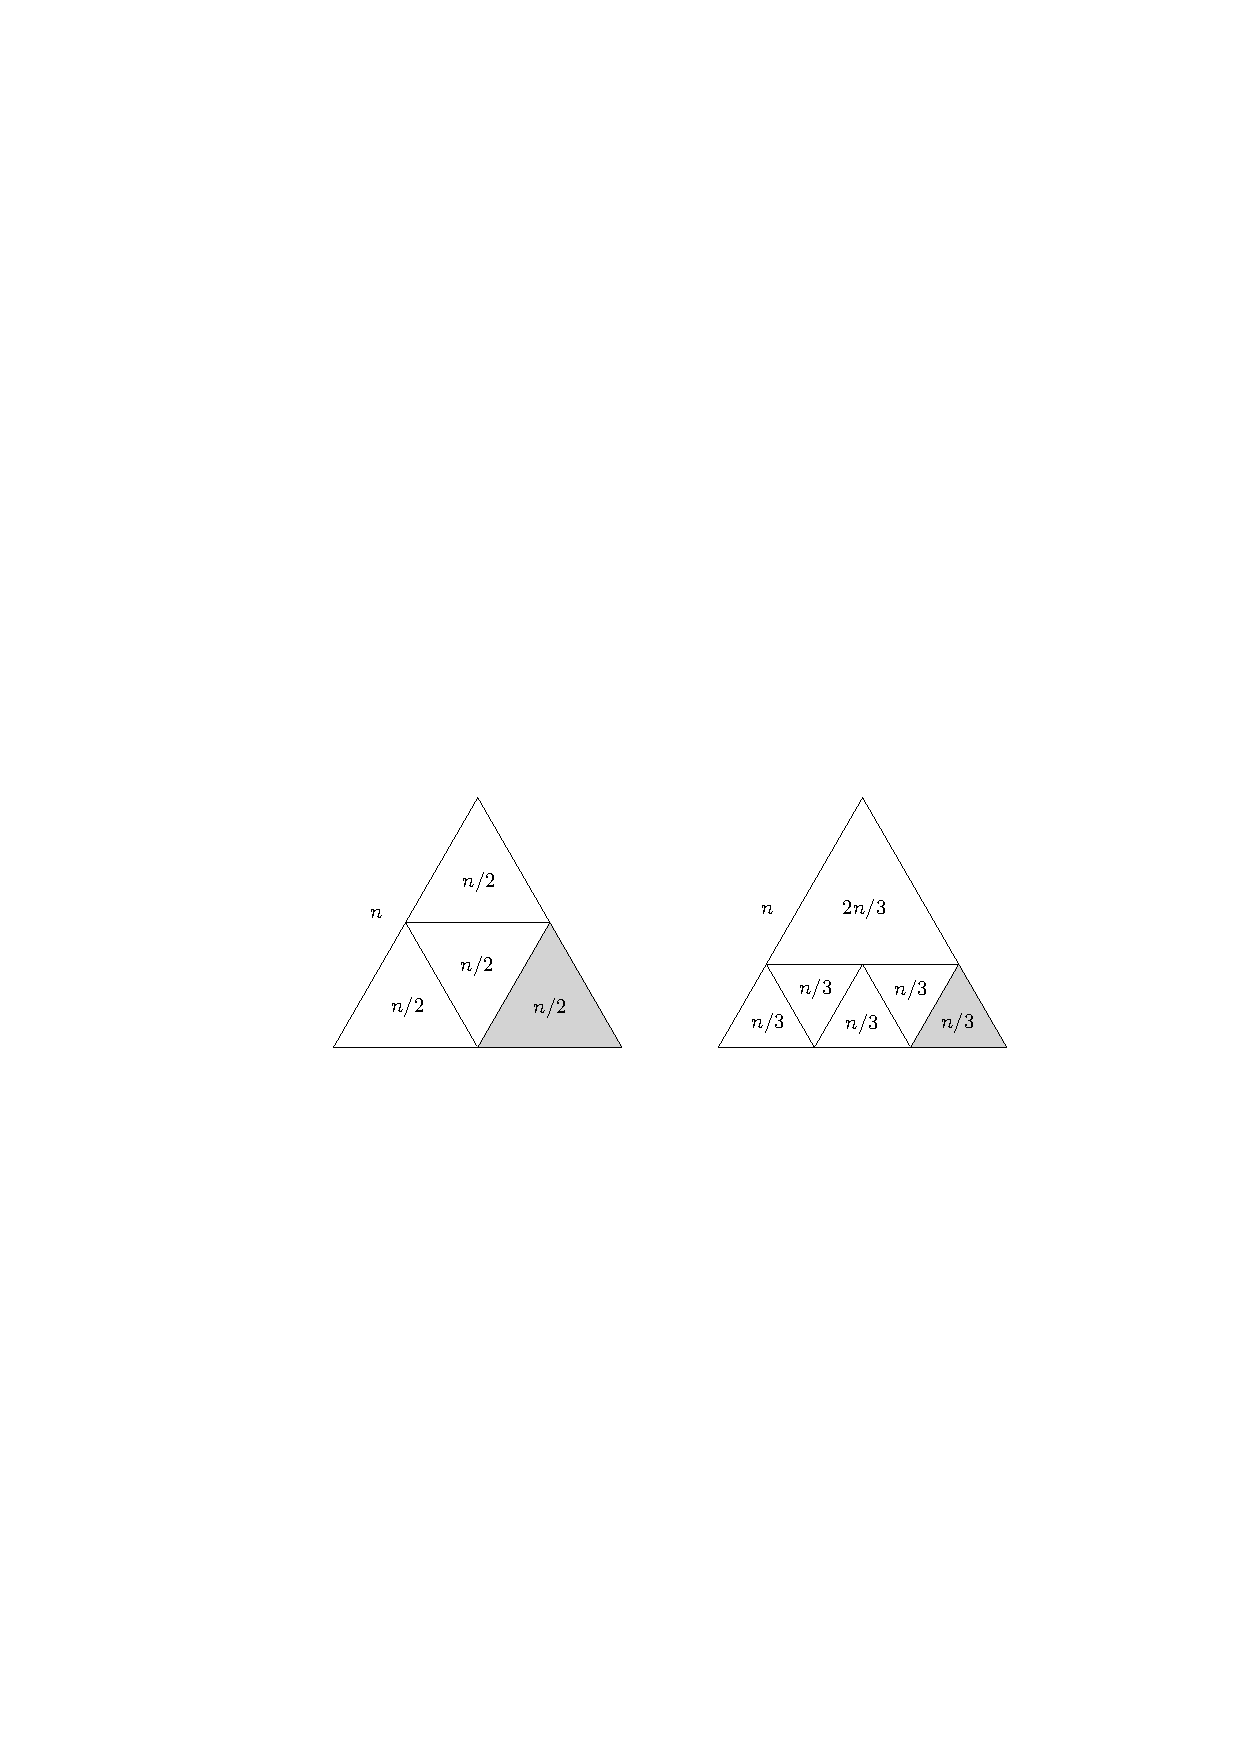
\includegraphics[width=0.8\textwidth]{img/triangle23.pdf}
\caption{Dissecting a triangle of side divisible by 2 and 3.}
\label{fig:triangle23}
\end{figure}

Steps (B1) and (B2) are illustrated on Figure \ref{fig:triangle23}. In (B3) we always use a prime dissection, therefore the resulting dissection is also prime. Clearly it is also $\circledast$-free.

Let us count the number of triangles used. If $r > 1$, then
\cosyalig{
	\hat t(n)
		&< 3p + 5q + 5\log_2(r) \\
		&< 5p \log_2(2) + 5q \log_2(3) + 5 \log_2(r) \\
		&= 5 \log_2(2^p3^qr) = 5 \log_2(n).
}
If $r=1$, then $\hat t(n) \leq 3p + 5q + 1$ and
\cosyalig{
	3p + 5q + 1 &< 5 \log_2(2^p3^q) = 5\log_2(n) \qquad \Leftrightarrow \\
	5q + 1 &< 2p + 5q \log_2(3) \qquad \Leftrightarrow \\
	1 &< 2p + (5\log_2(3)-5)q,
}
which holds every time at least one of $p,q$ is nonzero.
\end{proof}

%%%
%%%
%%%
\section{Triangle dissections and latin bitrades}
\label{sec:dissections-and-bitrades}

There is an interesting connection between triangle dissections and latin bitrades, first noted by Drápal \cite{Drapal91}. Let us begin with parametrization of a triangle dissection.

Consider a plane $\rho$ defined by $x+y+z=0$ in 3-dimensional Euclidean space. The planes with one fixed integer coordinate $x=k$, $y=k$, $z=k$ intersect with $\rho$, and lines of the intersections form a triangular grid.

We identify vector $(x_0, y_0, z_0)$ with the triangle bounded by lines $x=x_0$, $y=y_0$ and $z=z_0$. The number $|x_0+y_0+z_0|$ is the size (or side) of the triangle. Degenerate triangles of size 0 are points in the plane $\rho$.

\begin{figure}[htb]
\centering
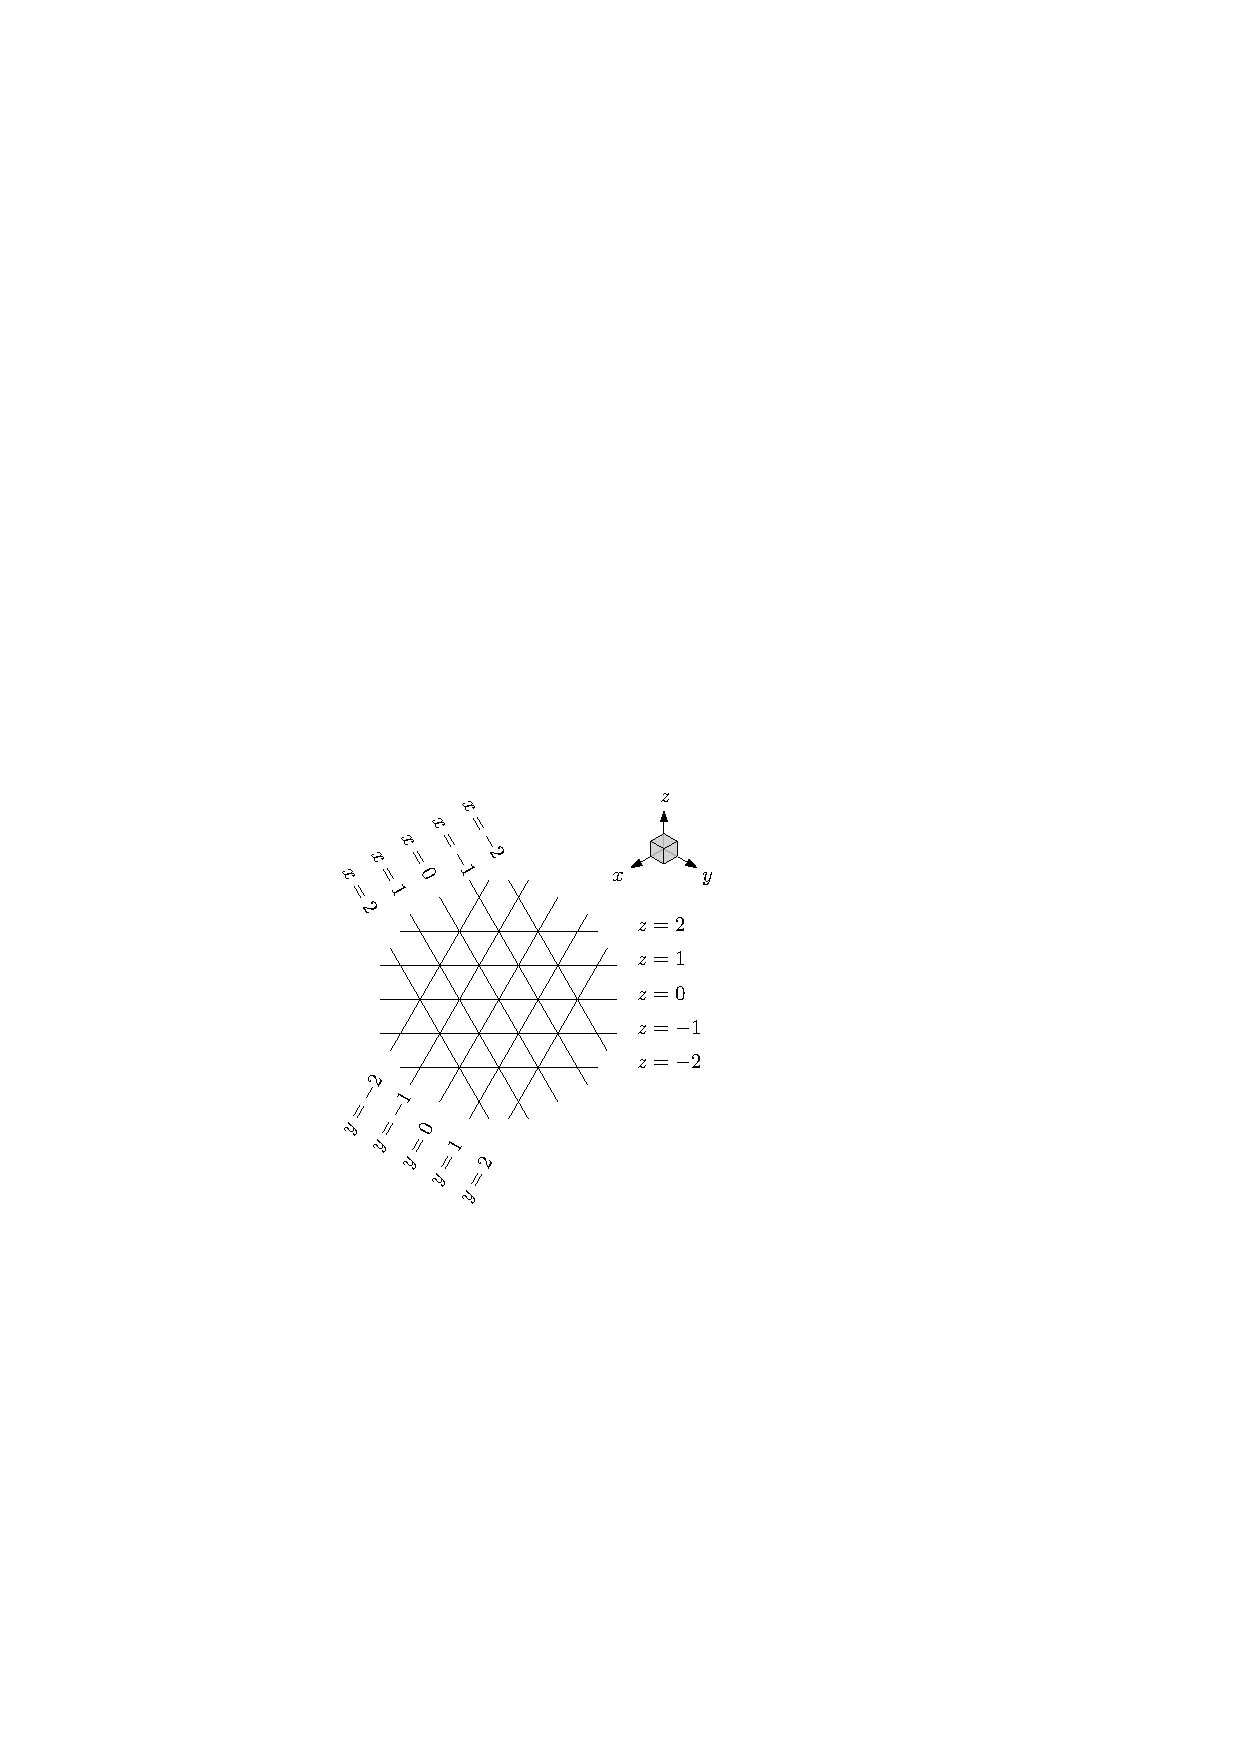
\includegraphics[height=14em]{img/trigrid.pdf}
\caption{Triangular grid in the plane $x+y+z=0$.}
\label{fig:trigrid}
\end{figure}

Now, we can embed a triangle dissection into the grid by choosing its position and orientation.

\begin{defn}
For a dissection $\D$ of a triangle $\Delta$ embedded in the plane $x+y+z=0$ define sets of vectors $T^*$, $T^\vartriangle$ such that
\begin{cosyitemize}
	\item $T^*$ is the set of vertices of the triangles in the dissection, with the vertices of $\Delta$ excluded and $\Delta$ itself included;
	\item $T^\vartriangle$ is the set of triangles in the dissection.
\end{cosyitemize}%
We call $(T^*, T^\vartriangle)$ \emph{an embedding of the dissection $\D$.}
\end{defn}

\begin{exmp} See Figure \ref{fig:arrows}.
\begin{figure}[htb]
	\centering
	\begin{minipage}{.43\linewidth}
		\centering
		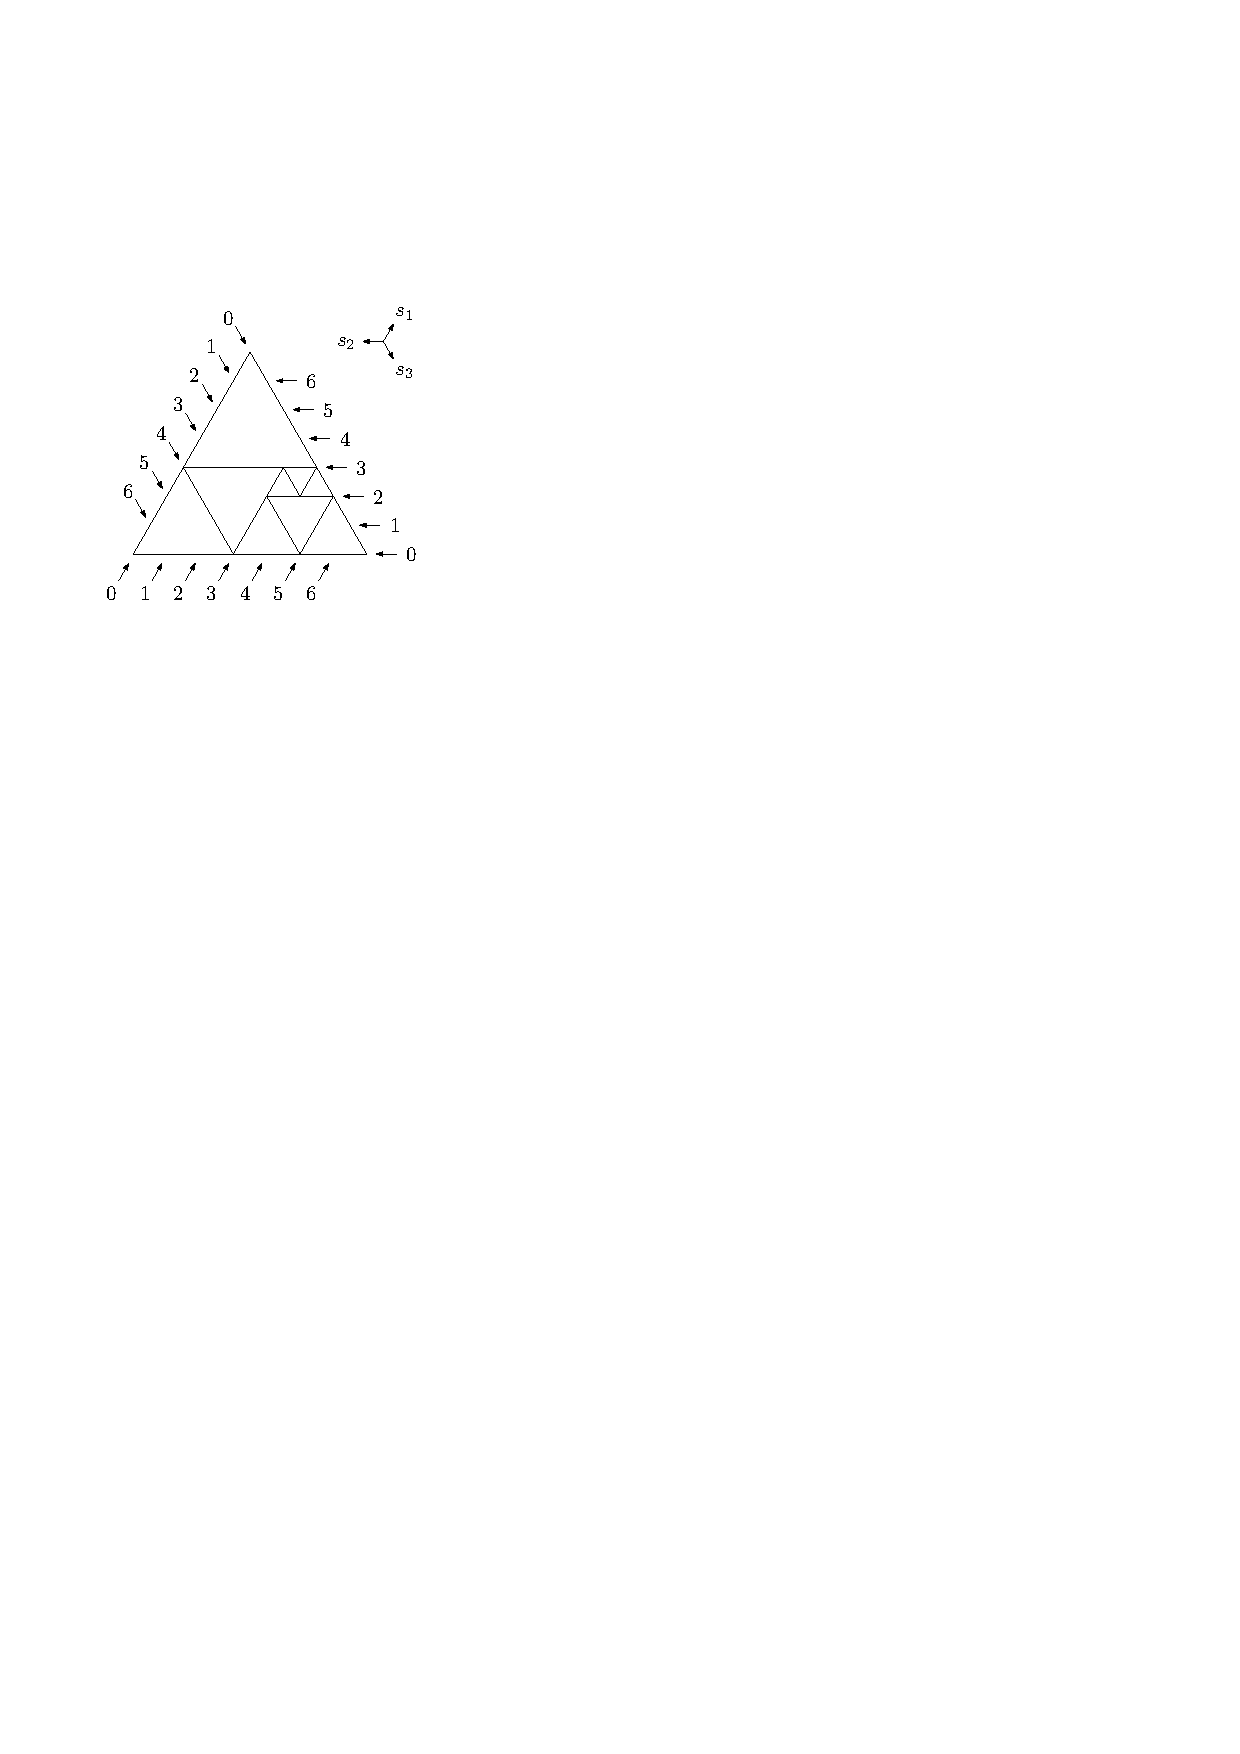
\includegraphics[width=0.9\textwidth]{img/arrows.pdf}
	\end{minipage}
	\hspace{.1\linewidth}
	\begin{minipage}{.16\linewidth}
		\begin{align*}
			\begin{array}{c}
				T^* \\ \hline
				(0,0,-7) \\
				(4,0,-4) \\
				(1,3,-4) \\
				(0,4,-4) \\
				(1,4,-5) \\
				(2,3,-5) \\
				(0,5,-5) \\
				(4,3,-7) \\
				(2,5,-7)
			\end{array}
		\end{align*}
	\end{minipage}
	\hspace{.04\linewidth}
	\begin{minipage}{.16\linewidth}
		\begin{align*}
			\begin{array}{c}
				T^\vartriangle \\ \hline
				(0,0,-4) \\
				(4,0,-7) \\
				(1,3,-5) \\
				(0,4,-5) \\
				(1,4,-4) \\
				(2,3,-7) \\
				(0,5,-7) \\
				(4,3,-4) \\
				(2,5,-5)
			\end{array}
		\end{align*}
	\end{minipage}
	\caption{Construction of $T^*$ and $T^\vartriangle$ from a triangulation.}
	\label{fig:arrows}
\end{figure}
\end{exmp}%

\begin{lem}
\label{lem:embedding-bitrade-main-class}
Let $\D$ be a $\circledast$-free triangle dissection. Then any embedding $(T^*, T^\vartriangle)$ of the dissection $\D$ is a latin bitrade. All such latin bitrades are from the same main class.
\end{lem}
\begin{proof}
 $(T^*, T^\vartriangle)$ is a bitrade straightforwardly from $\circledast$-freeness. Translation of the triangle corresponds to isotopy and rotation by multiples of $\pi/3$ to conjugacy, therefore the bitrades are from the same main class.
\end{proof}

Let us point out that we use two different notions of embedding -- embedding of a latin bitrade in a group is a homotopy, whereas embedding of a $\circledast$-free dissection (in the plane $x+y+z=0$) is a latin bitrade. 

Let $\Delta_n$ denote a triangle of side~$n$.

\begin{lem}
\label{lem:gdist-leq-tn}
$\gdist(n) \leq t(n)$.
\end{lem}
\begin{proof}
Let us have a $\circledast$-free dissection of $\Delta_n$ into $t(n)$ triangles. We claim that the map
\cosyalign{
	h:(x,y,z) \mapsto \big((x \bmod n), (y \bmod n), (z \bmod n)\big)
}%
is an embedding of $T^*$ into $\Z_n$, which would prove the statement.

Since the size of the triangle is $n$, it follows easily that $h$ is injective. Because $|x+y+z| \in \{0,n\}$ for $(x,y,z)\in T^*$, also $x+y+z \equiv 0 \pmod n$ holds and $h$ is a homotopy into $\Z_n$.
\end{proof}

\begin{lem}
\label{lem:gdist-n-leq-gdist-p}
If $p$ is a prime factor of $n$, then $\gdist(n) \leq \gdist(p)$.
\end{lem}%
\begin{proof}
Clearly if $H$ is a subgroup of $G$, then $\gdist(G) \leq \gdist(H)$. The rest follows from Cauchy's theorem.
\end{proof}

Finally, we have proved everything needed for our main result -- the proof of Conjecture \ref{conj:main}:

\begin{thm}
\label{cor:conj-proof}
Let $n \geq 2$ and $p$ be the smallest prime factor of $n$. Then
\cosyalign{
	3 \log_3(p) \leq \gdist(n) < 5 \log_2(p).
}
\end{thm}%
\begin{proof}
The lower bound is Theorem \ref{thm:lower-bound}. For the upper bound, combine Lemmas \ref{lem:gdist-n-leq-gdist-p}, \ref{lem:gdist-leq-tn} and Theorem \ref{thm:t-log-bound} to get
\cosyalign{
	\gdist(n) \leq \gdist(p) \leq t(p) = \hat t(p) < 5 \log_2(n).
}
\end{proof}

\begin{cor}
\label{cor:constants}
Let $n \geq 2$ and $p$ be the smallest prime factor of $n$. Then
\cosyalign{
	3 \log_3(e) \leq \frac{\gdist(n)}{\log(p)} < 5 \log_2(e).
}
\end{cor}%

%%%
%%%
%%%
\section{Families of logarithmic dissections}
\label{sec:other-log-dissections}

In previous sections we have seen how to use a logarithmic dissection into squares to get a logarithmic dissection into triangles. While the method presented gives the best results that we are aware of, in this section we show how it can be generalized, as it can possibly lead to ideas, which might be helpful in improving the upper bound in Corollary \ref{cor:constants}.

It seems that the main difficulty in doing so is to get a dissection of any shape of ``size $n$'' into $c \log(n)$ triangles for a good constant $c$. The additional requirements on $\circledast$-freeness, primality and modification of the dissection into a dissection of a triangle seem to be more of a technical detail. Indeed, in our earlier approach in this chapter, we ensured $\circledast$-freeness by introducing padded rectangle dissections; primality by taking an extra step in dissecting triangles of size $2k$ and $3k$; and a triangle dissection by adding two triangles to a dissection of a parallelogram.

For these reasons, and for simplicity of the argument, in this section we relax the $\circledast$-freeness and primality conditions on the dissections.

\bigskip

Let us sketch the method first. A convex hexagon, which we call \emph{core}, defines a dissection of a parallelogram into the core, 6 triangles and a smaller parallelogram. The sizes of the parallelograms depend on the shape of the core, and if chosen appropriately, the smaller parallelogram can be dissected recursively.

In the following, all shapes considered are aligned in a grid formed by unit equilateral triangles, i.e. all lengths are integer and all angles are multiples of $\pi/3$.

\begin{defn}
A convex hexagon $H$ in a unit triangular grid is \emph{a core}. Let us denote its side lengths consecutively by $a_1,\dots,a_6 \in \Z_0^+$. We allow the hexagon to be degenerate, i.e. some of its sides can be zero. From the properties of such a hexagon, the following holds:
\cosyalign{
	a_1 + a_2 &= a_4 + a_5 =: \alpha \\
	a_2 + a_3 &= a_5 + a_6 =: \beta \\
	a_3 + a_4 &= a_6 + a_1 =: \gamma
}
Therefore the hexagon is uniquely specified by a 4-tuple $(a_1, \alpha, \beta, \gamma)$. We will often identify $H = (a_1, \alpha, \beta, \gamma)$.
\end{defn}

Note that not every 4-tuple specifies a valid hexagon. Also note that
\cosyalign{
	a_1 + \dots + a_6 = \alpha + \beta +\gamma
}%
is perimeter of a core.

\begin{defn}
\emph{A shape S} is a union of finitely many unit triangles in the triangular grid. Let us denote by $t(S)$ the minimal number of triangles needed to dissect the shape $S$, and let $t_d(n)$ denote $t(S)$ for a parallelogram S of size $n \times (n+d)$.
\end{defn}

We kindly ask the reader to extrapolate the formal definition of a dissection from Definition \ref{defn:triangle-dissection}.

\begin{lem}
\label{lem:core-tiling}
Let $H = (a_1, \alpha, \beta, \gamma)$ be a core and $k$ a positive integer. Set $n = 2k+a_1+\alpha+\beta$ and denote by $P$ and $P'$ parallelograms of sizes $n\times(n+\gamma)$ and $k\times(k+\alpha+\beta+\gamma)$. Then there exists a dissection of $P$ into $H$, $P'$ and six triangles. Therefore
\cosyalign{
	t_\gamma(n) \leq 6 + t(H) + t_{\alpha+\beta+\gamma}(k)
}
\end{lem}
\begin{proof}
See Figure \ref{fig:core-tiling1}.
\end{proof}

\begin{figure}[htb]
\centering
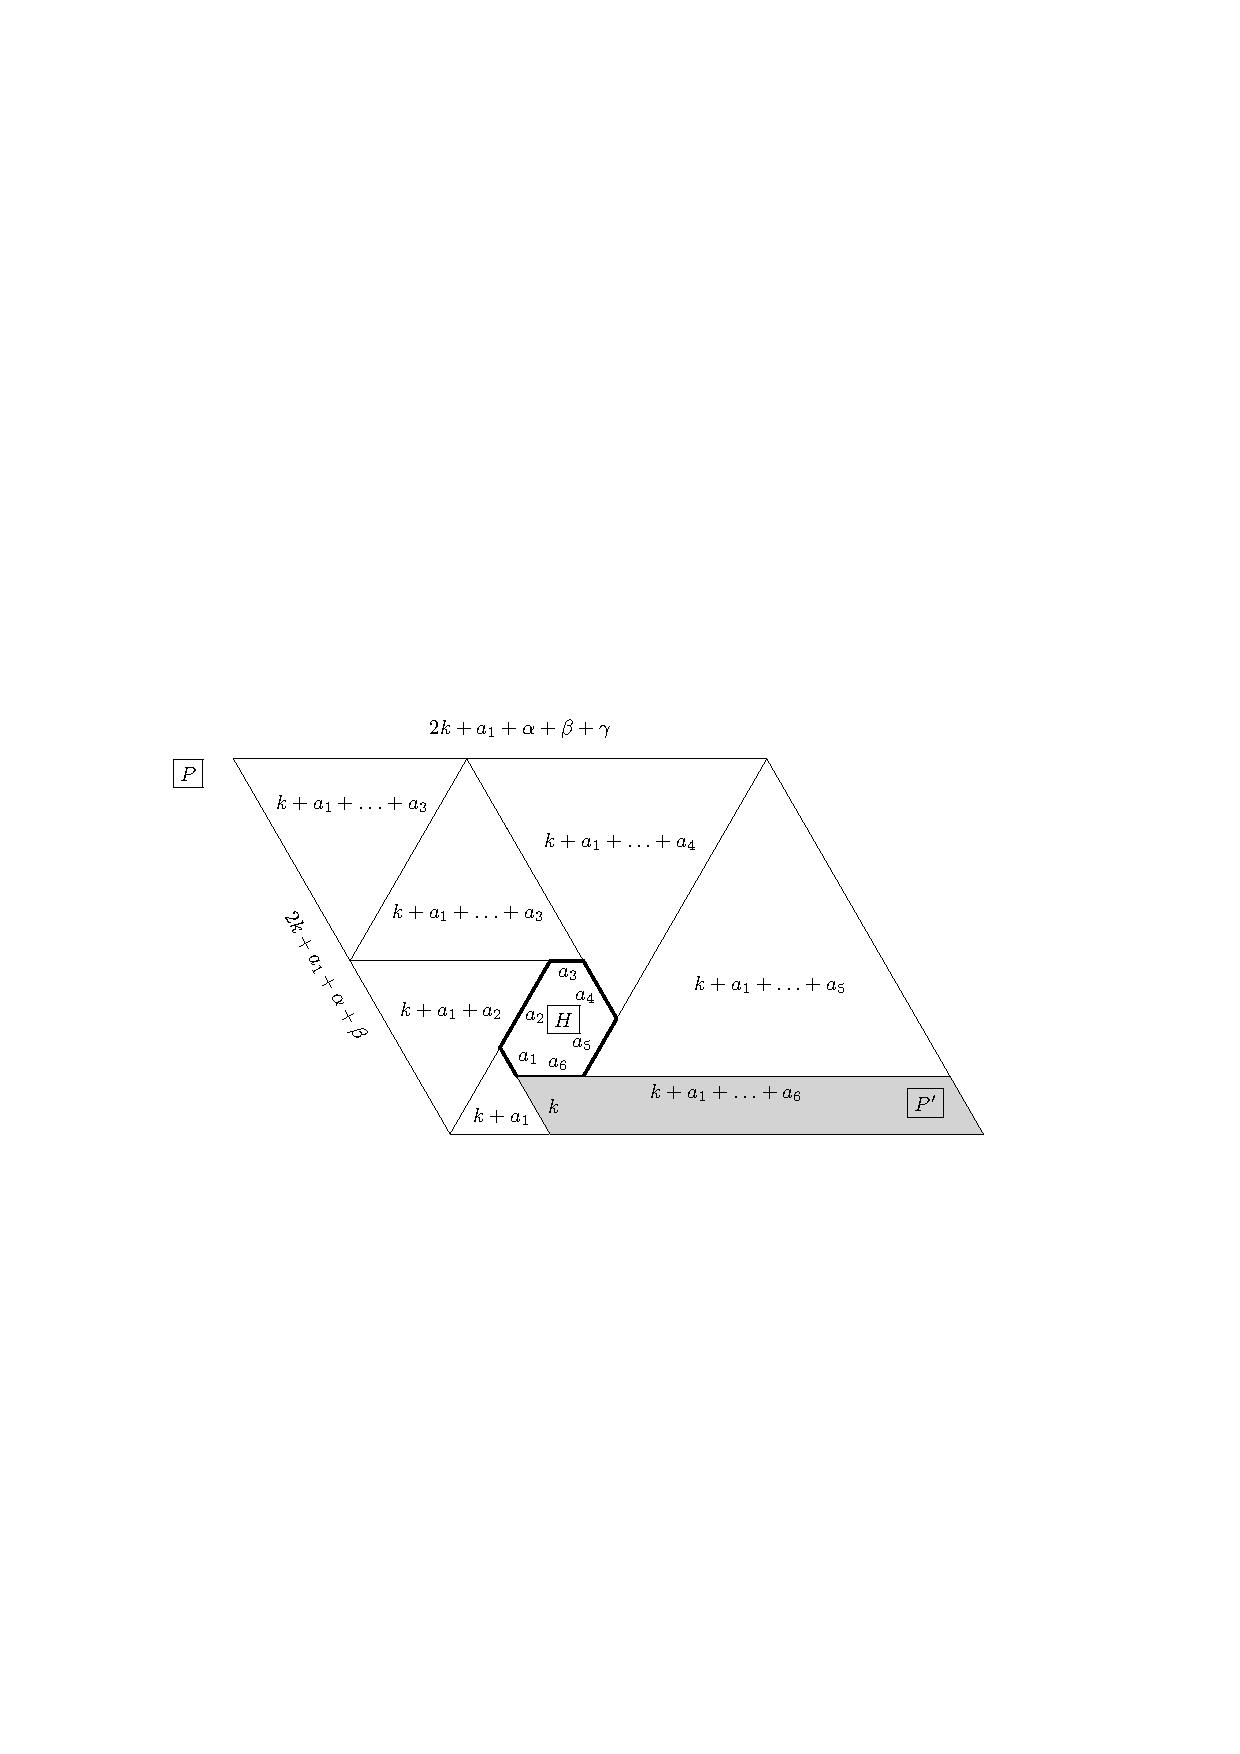
\includegraphics[width=0.9\textwidth]{img/core_tiling1.pdf}
\caption{Dissection of a parallelogram into convex hexagon, six triangles and a parallelogram.}
\label{fig:core-tiling1}
\end{figure}

Now, let us set the variables such that we can use the tiling recursively. First, fix $\gamma$ and $\alpha+\beta+\gamma$, so that $P$ and $P'$ are always of sizes $n \times (n+\gamma)$ and $k \times (k+\alpha+\beta+\gamma)$. Next, we would like to tile $P$ with tiles of sides which are multiples of an integer $d$. Therefore reset $k := dk$ and set $\alpha+\beta+\gamma = d\gamma$. In this setting,
\cosyalig{
	&P \textrm{ is of size } n \times (n + \gamma)\textrm{, and} \\
	&P' \textrm{ is of size } dk \times (dk + d\gamma)
}
with $n = 2dk + (d-1)\gamma + a_1$.

Finally, if $n$ can be of any integer value (possibly for $n > n_0$ for some $n_0$), we can use the dissection recursively. Since $k$ can be any integer, it suffices for $(d-1)\gamma + a_1$ to go through all remainders modulo $2d$. The term $(d-1)\gamma$ is a constant, therefore $a_1$ must be such. Because $a_1$ is nonnegative and $a_1 \leq \gamma = a_1 + a_6$, this gives us the final requirement $2d-1 \leq \gamma$.

\begin{lem}
\label{lem:t-gamma-n}

Let $d,\gamma \geq 2$ be integers such that $2d-1 \leq \gamma$. Then there exists $n_0$ and a constant $T$ such that
\cosyalign{
	t_\gamma(n) \leq 6 + T + t_\gamma(k)
}%
for $n > n_0$ and some $k < n/(2d)$.
\end{lem}
\begin{proof}
For $a \in [0,2d)$ denote
\cosyalig{
	T_a = \min \{t(H) \mid\ &H=(a_1,\alpha,\beta,\gamma) \mbox{ is a core, } \\
	&\alpha+\beta+\gamma = d\gamma,  \\
	&a_1 \equiv a \pmod{2d}\}
}%
and define $T = \max \{T_a \mid a \in [0,2d)\}$. $T_a$ is well-defined for every $a$ -- it can be easily seen that there always exists a core with required parameters.

Set $n_0 = 2d+d\gamma$ and take $n > n_0$. Then there is $a \in [0,2d)$ such that $n \equiv (d-1)\gamma + a \pmod{2d}$ and a core $H=(a_1,\alpha,\beta,\gamma)$ which we have chosen such that $t(H) = T_a$.

Now, $n$ can be written as $2dk + (d-1)\gamma + a_1$ for a positive integer $k$. Plugging into Lemma \ref{lem:core-tiling} we get
\cosyalign{
	t_\gamma(n) \leq 6 + t(H) + t_{d\gamma}(dk) \leq 6 + T + t_\gamma(k).
}%
Clearly $k < n/(2d)$, which completes the proof.
\end{proof}

\begin{cor}
\label{cor:log-t-gamma-n}
Let $d,\gamma$ be as in Lemma \ref{lem:t-gamma-n}. Then there exist constants $T,C$ such that
\cosyalign{
	t_\gamma(n) \leq (6+T) \log_{2d}(n) + C.
}%
\end{cor}%

\begin{defn}
Let us call the dissection constructed in the proof of Lemma \ref{lem:t-gamma-n} \emph{a core dissection} of a parallelogram $n \times (n+\gamma)$. Denote the number of triangles used by $\bar t_\gamma(n)$.
\end{defn}

\begin{exmp}
Let us choose $d=2$ and $\gamma=3$, they meet the conditiion $2d-1 \leq \gamma$. Consider the cores on Figure \ref{fig:core-kk3}, they have to have perimeter $d\gamma = 6$.

We chose $a_1 \in \{0,1,2,3\}$ as this is the only choice such that $a_1 \leq \gamma$ and $a_1$ runs through all remainders modulo $2d=4$. We can set $T=4$ and from Corollary \ref{cor:log-t-gamma-n} we have
\cosyalign{
	t_3(n) \leq 10 \log_{4}(n) + C = 5 \log_2(n) + C
}%
for a constant $C$. The resulting tiling is in fact the tiling from Section \ref{sec:log-rectangle}  with every square diagonally cut in halves.

\begin{figure}[htb]
\centering
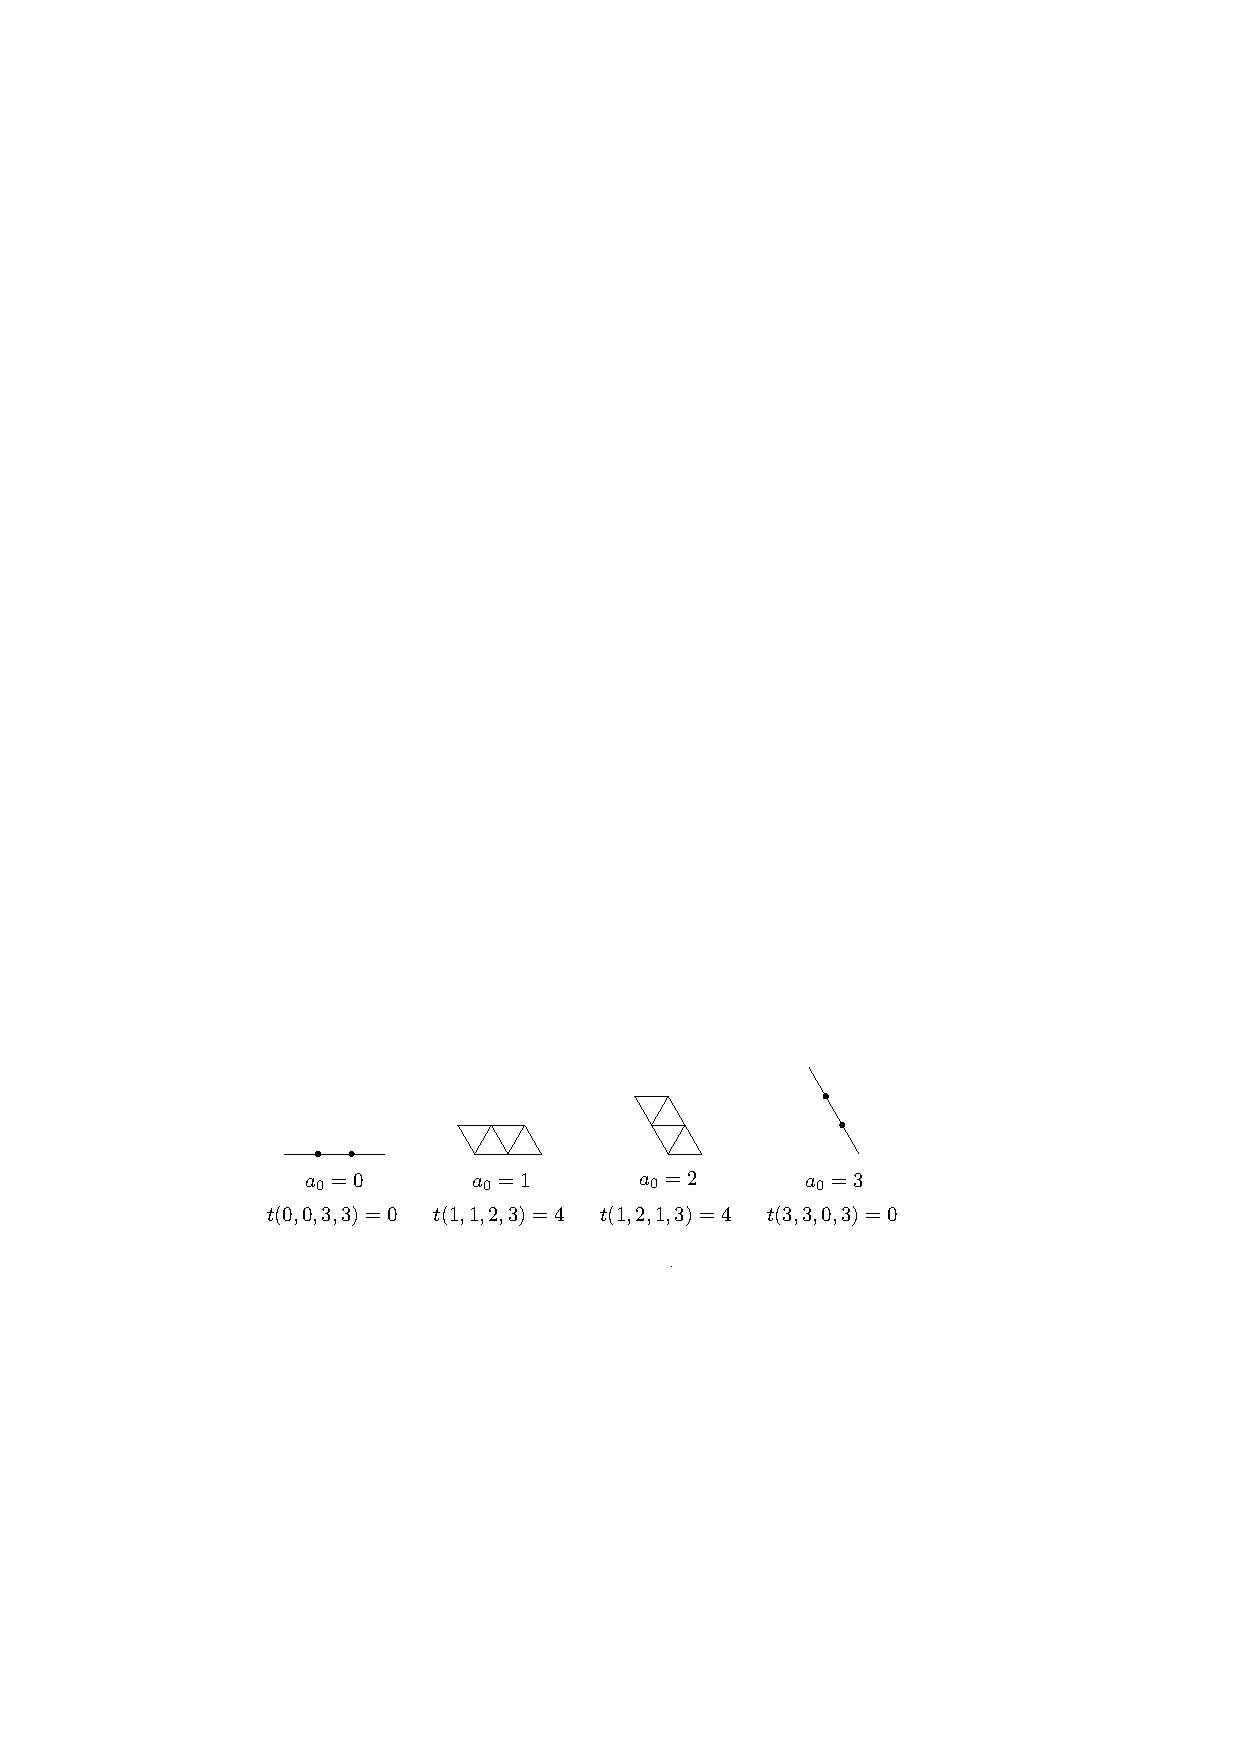
\includegraphics[width=0.8\textwidth]{img/example_core_kk3.pdf}
\caption{Cores for $d=2$, $\gamma=3$. We denote the size of tiling of the corresponding core briefly by $t(a_1,\alpha,\beta,\gamma)$.}
\label{fig:core-kk3}
\end{figure}
\end{exmp}%

It would be desirable to construct a chain of better and better dissections that converge to the expected bound proposed in Chapter \ref{chap:bounds}. However, the following lemmas show that using core dissections, this is not possible.

\begin{lem}
\label{lem:core-dissection-bound}
Let $H = (a_1, \alpha, \beta, \gamma)$ be a core of perimeter $d\gamma$ and $a_1 \ne 0 \ne a_6$. Then $t(H) \geq d$.
\end{lem}
\begin{proof}
Let us denote by $a_1, \dots, a_6$ the corresponding sides instead of their lengths. Distance between the pair of parallel lines $a_2, a_5$ is $\frac{\sqrt{3}}{2}\gamma$, and therefore the largest triangle that can fit in $H$ can be of side $\gamma$. Therefore to cover the sides $a_2$ and $a_5$ we have to use at least $(a_2+a_5)/\gamma = (d\gamma-2\gamma)/\gamma = d-2$ triangles.

Since $a_1 \ne 0 \ne a_6$, we have to use at least one more triangle to cover each of these sides. These triangles have to be distinct from those lying on sides $a_2$ and $a_5$, hence $t(H) \geq d$.

\begin{figure}[htb]
\centering
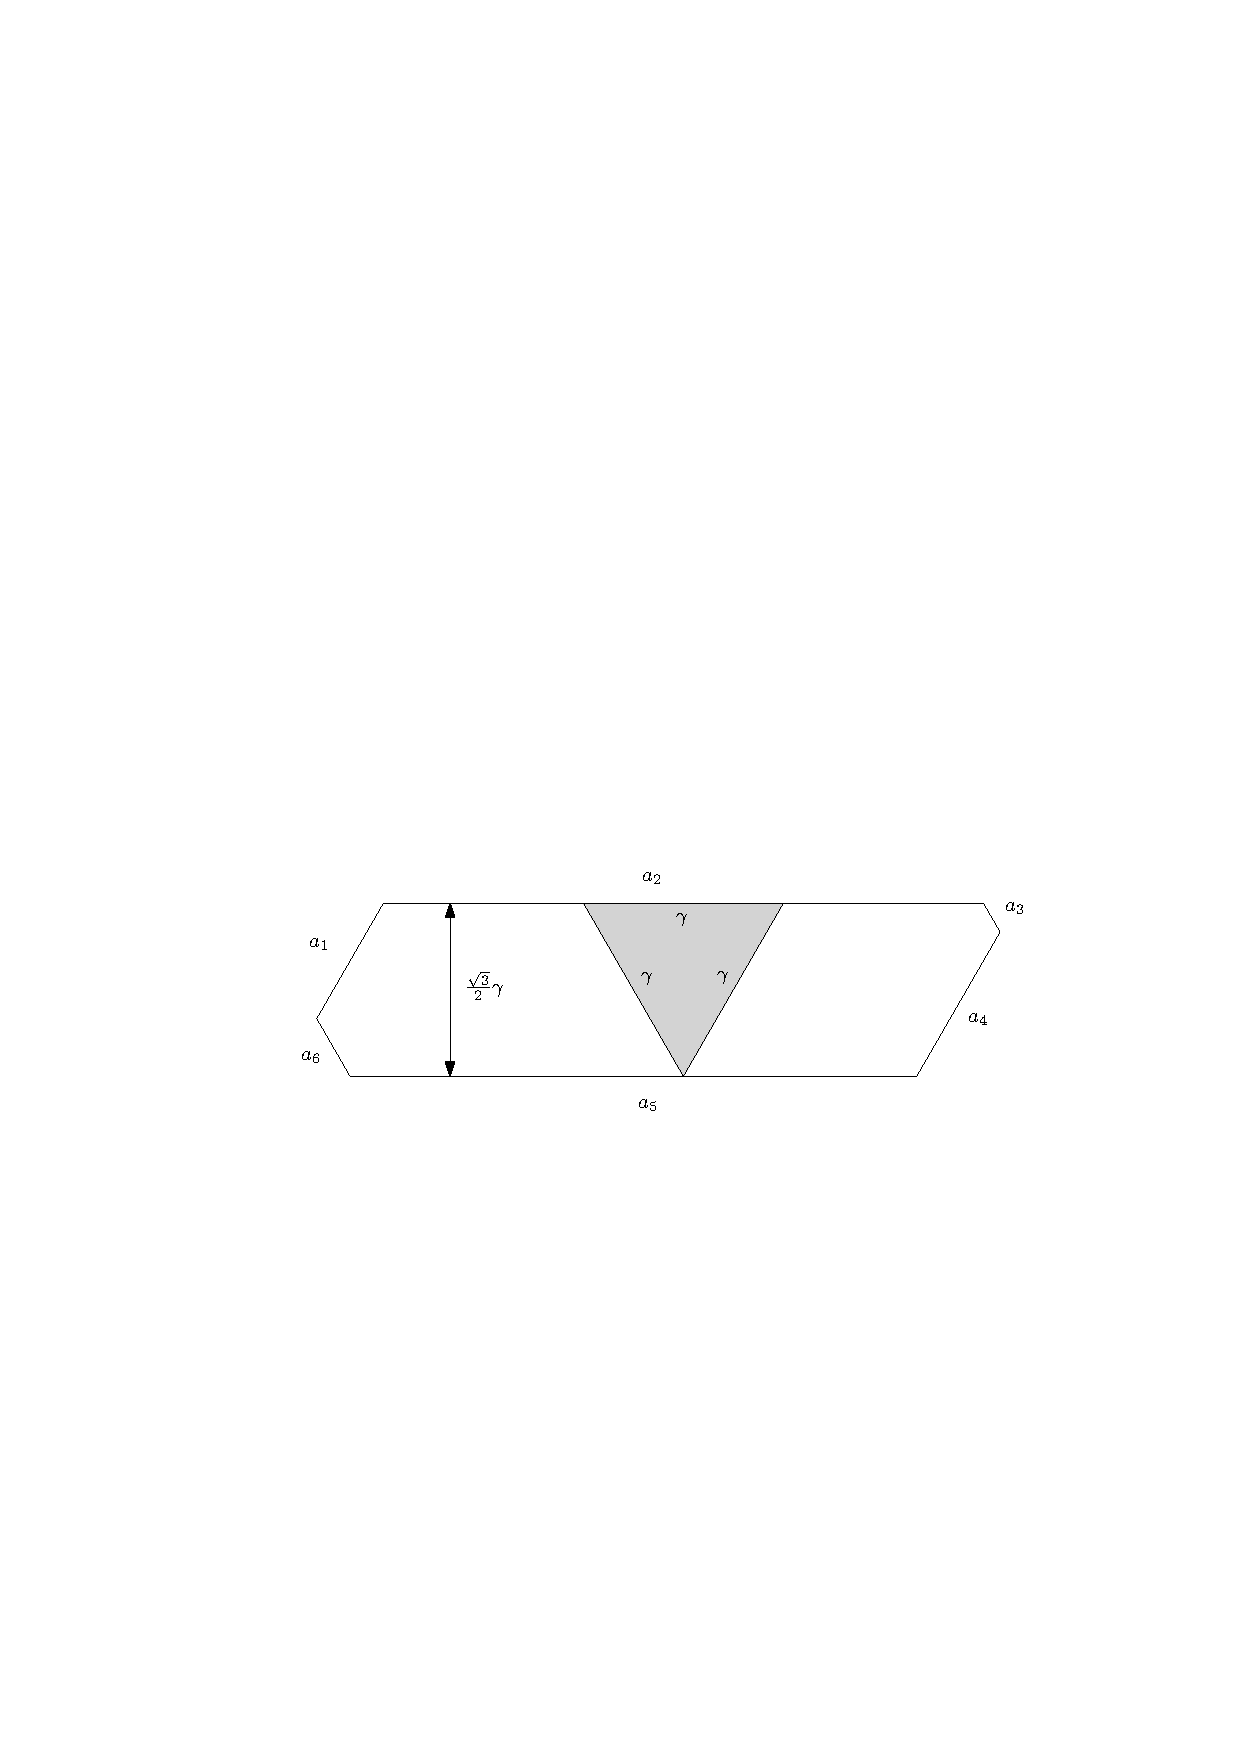
\includegraphics[width=0.8\textwidth]{img/core_tiling_lower_bound.pdf}
\caption{Tiling a core of perimeter $d\gamma$.}
\label{fig:core-tiling-lower-bound}
\end{figure}\end{proof}

\begin{lem}
\label{lem:core-disection-lower-bound}
Let $d,\gamma$ be as in Lemma \ref{lem:t-gamma-n}. Then
\cosyalign{
	\bar t_\gamma(n) \geq (6+d) \log_{2d}(n).
}
\end{lem}%
\begin{proof}
Let us have $T$, $d$ as in the proof of Lemma \ref{lem:t-gamma-n}. By Lemma \ref{lem:core-dissection-bound}, $T \geq d$. The result now follows by plugging into Corollary \ref{cor:log-t-gamma-n}.
\end{proof}

Let us compare core dissections with the dissection into $5 \log_2(n)$ triangles. Because we compare dissections into asymptotically logarithmically many triangles, we are interested in the ratio over $\log(n)$. Therefore the necessary condition for a core dissection into $\hat t_\gamma(n)$ triangles to be better is
\begin{align}
	& &\frac{\bar t_\gamma(n)}{\log (n)} &< \frac{5 \log_2(n)}{\log(n)} \hspace{8em} \\
	(Lemma\ \ref{lem:core-disection-lower-bound})&\Rightarrow & \frac{6+d}{\log(2d)} &< \frac{5}{\log(2)} \\
	&\Leftrightarrow & 2^{6+d} &< (2d)^5 \\
	&\Leftrightarrow &  2 ^ {1+d} &< d^5.
\end{align}
The last inequality has integer solutions only for $d \leq 20$. Therefore there can be only finitely many better core dissections (for fixed $d$ there are finitely many, the only significant variable is the positive integer $T$ in the estimate $(6+T)\log_{2d}(n) + C$).

It was not our primary goal to establish that the dissection into $5 \log(n)$ triangles is the best in any sense. However, we conjecture that it actually is among all core dissections.






% Ukázka použití některých konstrukcí LateXu (odkomentujte, chcete-li)
% %%% Ukázka použití některých konstrukcí LaTeXu

\subsection{Ukázka \LaTeX{}u}
\label{ssec:ukazka}

This short subsection serves as an~example of basic \LaTeX{} constructs,
which can be useful for writing a~thesis.

Let us start with lists:

\begin{itemize}
\item The logo of Matfyz is displayed in figure~\ref{fig:mff}.
\item This is subsection~\ref{ssec:ukazka}.
\item Citing literature~\cite{lamport94}.
\end{itemize}

Different kinds of dashes:
red-black (short),
pages 16--22 (middle),
$45-44$ (minus),
and this is --- as you could have expected --- a~sentence-level dash,
which is the longest.
(Note that we have follwed \verb|a| by a~tilde instead of a~space
to avoid line breaks at that place.)

\newtheorem{theorem}{Theorem}
\newtheorem*{define}{Definition}	% Definice nečíslujeme, proto "*"

\begin{define}
A~{\sl Tree} is a connected graph with no cycles.
\end{define}

\begin{theorem}
This theorem is false.
\end{theorem}

\begin{proof}
False theorems do not have proofs.
\end{proof}

\begin{figure}
	\centering
	
\includegraphics[width=30mm]{../img/logo.eps}
	\caption{Logo of MFF UK}
	\label{fig:mff}
\end{figure}


\chapter*{Conclusion}
\addcontentsline{toc}{chapter}{Conclusion}


%%% Seznam použité literatury
%%% Seznam použité literatury je zpracován podle platných standardů. Povinnou citační
%%% normou pro diplomovou práci je ISO 690. Jména časopisů lze uvádět zkráceně, ale jen
%%% v kodifikované podobě. Všechny použité zdroje a prameny musí být řádně citovány.

\addcontentsline{toc}{chapter}{Bibliography}
\bibliography{bibliography.bib}{}
%\bibliographystyle{chicago}

\bibliographystyle{plain}


%\def\bibname{Bibliography}
%\begin{thebibliography}{99}

%\bibitem{lamport94}
%  {\sc Lamport,} Leslie.
%  \emph{\LaTeX: A Document Preparation System}.
%  2. vydání.
%  Massachusetts: Addison Wesley, 1994.
%  ISBN 0-201-52983-1.

%\end{thebibliography}


%%% Tabulky v diplomové práci, existují-li.
\chapwithtoc{List of Tables}

%%% Použité zkratky v diplomové práci, existují-li, včetně jejich vysvětlení.
\chapwithtoc{List of Abbreviations}

%%% Přílohy k diplomové práci, existují-li (různé dodatky jako výpisy programů,
%%% diagramy apod.). Každá příloha musí být alespoň jednou odkazována z vlastního
%%% textu práce. Přílohy se číslují.
\chapwithtoc{Attachments}

\openright
\end{document}
